\chapter{Livello di collegamento}
\section{Introduzione}
Nel capitolo precedente si è visto che la comunicazione a livello di rete avviene tra host. Un datagramma è un'unità dati che può essere frammentata e riassemblata ma che in generale viene inviata da un host, che si trova da qualche parte nel mondo, ad un altro host, che si trova in qualche altra zona. Internet non è altro che una combinazione di reti unite assieme da dispositivi di collegamento (per esempio, router e switch). Se un datagramma deve viaggiare da un host ad un altro, deve quindi passare necessariamente attraverso tali reti.

\begin{Example}{Comunicazione a livello di collegamento}{}
    \textit{La figura mostra la comunicazione tra Gaia e Gabriele.}
    
    \begin{wrapfigure}{r}{0.45\textwidth}
        \vspace{-0.5cm}
        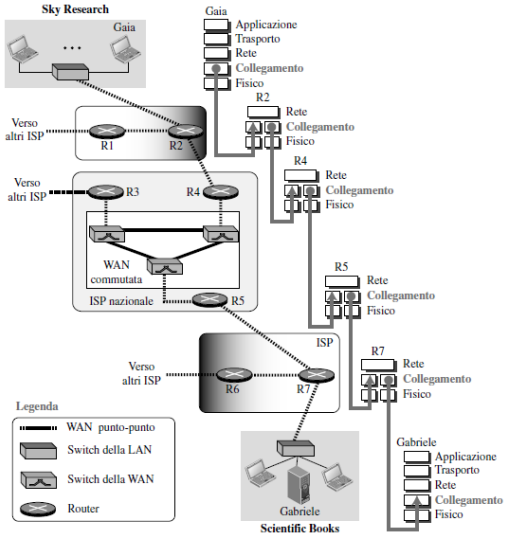
\includegraphics[width=0.45\textwidth]{images/liv-collegamento.PNG}
        \vspace{-0.5cm}
    \end{wrapfigure}
    
    Tuttavia, in questo caso, la comunicazione a livello di collegamento è composta da cinque connessioni logiche separate tra i diversi livelli di collegamento lungo il percorso tra i due host.

    Il livello di collegamento sul computer di Gaia comunica con quello sul router R2. Il livello di collegamento sul router R2 comunica con quello sul router R4, e così via. Infine, il livello di collegamento sul router R7 comunica con quello del computer di Gabriele. Solo un livello di collegamento è coinvolto alla sorgente e alla destinazione, a differenza dei router dove ne sono coinvolti due. Questo avviene poiché i computer di Gaia e Gabriele sono collegati ciascuno ad una sola rete, i router invece ricevono da una rete e trasmettono su un'altra.
\end{Example}

Anche se la comunicazione nei livelli di applicazione, trasporto e rete è end-to-end (cioè avviene, dal punto di vista logico, dall'host iniziale a quello finale), quella a livello di collegamento è invece da nodo a nodo. Come si è visto nei capitoli precedenti, un'unità di dati (cioè un pacchetto) trasmessa da un certo punto della rete per arrivare fino alla sua destinazione deve attraversare molte altre reti (LAN e WAN) collegate per mezzo di router. E' consuetudine riferirsi ai router e agli host alle due estremità come a nodi e alle reti nel mezzo come a collegamenti. Nella Figura \ref{fig:nodi-collegamenti} è possibile trovare la rappresentazione di un semplice percorso formato da soli sei nodi.

\begin{figure}[ht]
    \centering
    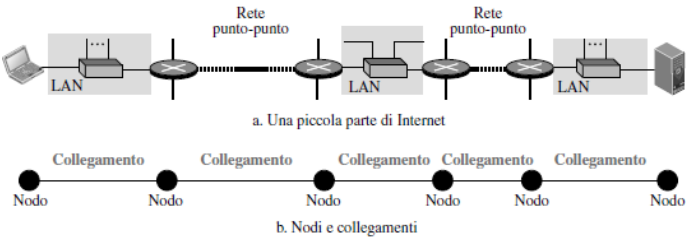
\includegraphics[width=11cm]{images/nodi-collegamenti.PNG}
    \caption{Nodi e collegamenti}
    \label{fig:nodi-collegamenti}
\end{figure}

Il primo nodo è l'host sorgente e l'ultimo è l'host di destinazione. Gli altri quattro nodi intermedi sono dei router. Il primo, il terzo e il quinto collegamento rappresentano tre LAN, il secondo e il quarto due WAN.

I nodi all'interno delle reti sono fisicamente collegati da un mezzo trasmissivo, come un cavo o l'aria. Compito del livello di collegamento è controllare come viene usato tale mezzo. Possiamo avere un livello di collegamento che utilizza l'intera capacità di un mezzo oppure solo parte della sua capacità. In altre parole, possiamo avere un collegamento punto-punto o un collegamento broadcast. In un collegamento punto-punto, il collegamento è dedicato a due soli dispositivi (mittente e ricevente). Viceversa, in un collegamento broadcast, il collegamento è condiviso tra varie coppie di dispositivi. Per esempio, quando due amici usano il telefono di casa per chiacchierare, stanno usando un collegamento punto-punto. Quando gli stessi due amici usano i loro telefoni cellulari, stanno usando un collegamento broadcast (visto che l'aria viene condivisa tra vari utilizzatori di cellulari).

Per comprendere meglio le funzionalità ed i servizi forniti dal livello di collegamento possiamo dividere questo livello in due sotto-livelli: il Data-Link Control (DLC) ed il controllo dell'accesso al mezzo trasmissivo (Media Access Control, MAC). Il sotto-livello di DLC si occupa di tutte le questioni comuni sia ai collegamenti punto-punto che a quelli broadcast. Il sotto-livello MAC si occupa invece solo degli aspetti specifici dei canali broadcast. 

\begin{figure}[ht]
    \centering
    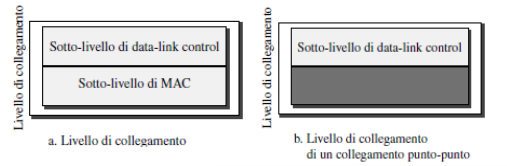
\includegraphics[width=9cm]{images/due-sottolivelli.PNG}
    \caption{Divisione del livello di collegamento in due sotto-livelli}
    \label{fig:due-sottolivelli}
\end{figure}

\subsection{Servizi offerti dal livello di collegamento}
Sebbene il servizio di base del livello di collegamento sia il trasporto di datagrammi
da un nodo a quello adiacente lungo un singolo canale di comunicazione, i dettagli
dei servizi forniti possono variare da un protocollo all’altro. I possibili servizi che
possono essere offerti dai protocolli a livello di collegamento includono i seguenti.
\begin{itemize}
    \item \textit{Framing.} Quasi tutti i protocolli incapsulano i datagrammi del livello di rete all’interno di un frame a livello di collegamento, prima di trasmetterlo. I frame sono costituiti da un campo dati, nel quale è inserito il datagramma, e da vari campi di intestazione. La struttura del frame è specificata dal protocollo.
    \item \textit{Accesso al collegamento.} Un protocollo che controlla l’accesso al mezzo trasmissivo (MAC, medium access control) specifica le regole con cui immettere i frame nel collegamento.
    \item \textit{Consegna affidabile.} I protocolli a livello di collegamento che forniscono un servizio di consegna affidabile garantiscono il trasporto senza errori di ciascun datagramma. Abbiamo già visto che anche alcuni protocolli di trasporto (come TCP) forniscono un servizio di consegna affidabile. Analogamente a quello del livello di trasporto, anche il servizio di consegna affidabile del livello di collegamento può essere realizzato attraverso acknowledgment e ritrasmissioni. Il servizio di consegna affidabile è spesso utilizzato per i collegamenti soggetti a elevati tassi di errore (per esempio i collegamenti wireless), allo scopo di correggere l’errore localmente, sul collegamento dove è avvenuto l’errore, piuttosto che costringere i protocolli di trasporto o di applicazione a procedere alla ritrasmissione dei dati dalla sorgente alla destinazione. Tuttavia, la consegna affidabile del livello di collegamento può essere considerata non necessaria nei collegamenti che presentano un basso numero di errori sui bit, come nel caso di collegamenti con fibra ottica, cavo coassiale e doppino, ragion per cui molti protocolli del livello di collegamento non implementano questo servizio.
    \item \textit{Controllo di flusso.} Così come avviene a livello trasporto, il controllo di flusso coordina la quantità di dati che può essere inviata prima di ricevere un riscontro. I concetti di fondo del controllo di flusso a livello di collegamento sono gli stessi del livello trasporto.
    \item \textit{Rilevazione e correzione degli errori.} Il nodo ricevente può decidere, erroneamente, che un bit in un frame sia 0 quando questo era stato trasmesso come 1, e viceversa. Gli errori di bit sono causati dall’attenuazione di segnale e dai disturbi elettromagnetici. Siccome non è utile inoltrare i datagrammi contenenti errori, molti protocolli del livello di collegamento forniscono un meccanismo per rilevarne la presenza. Ciò è possibile grazie all’inserimento, da parte del nodo trasmittente, di bit di controllo di errore all’interno del frame e all’esecuzione di un semplice controllo da parte del nodo ricevente. Anche il livello di trasporto e di rete di Internet fornisce una seppur limitata rilevazione degli errori: il checksum (Internet checksum). Il rilevamento degli errori a livello di collegamento è però solitamente più sofisticato, in quanto implementato in hardware. La correzione dell’errore è simile alla rilevazione degli errori, ma in più il nodo ricevente determina il punto preciso del frame in cui si è verificato l’errore (per poi correggerlo).

    Ogni volta che i bit fluiscono da un punto ad un altro sono soggetti a cambiamenti imprevedibili, a causa delle interferenze. Queste interferenze possono cambiare la forma del segnale e quindi alterare la ricezione dei bit. Il termine errore su un singolo bit (single-bit error) indica che un solo bit in una determinata unità di dati (ad esempio: un byte, un carattere o un pacchetto) è stato cambiato da 1 a 0 o viceversa. Il termine errore a ruffica (burst error) indica che 2 o più bit nell'unità di dati sono stati cambiati di valore.

    \begin{figure}[ht]
        \centering
        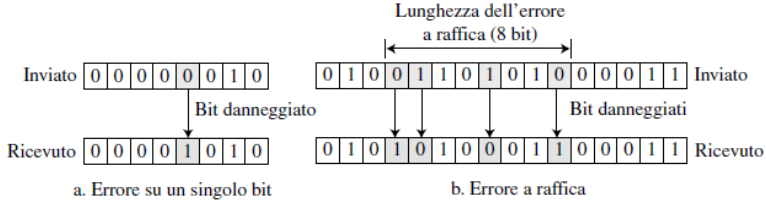
\includegraphics[width=11cm]{images/errori-bit-burst.PNG}
        \caption{Errore su un singolo bit ed errore a raffica}
        \label{fig:errori-bit-burst}
    \end{figure}
    
    La probabilità che avvenga un errore a raffica è più elevata rispetto a quella di un errore su un singolo bit, in quanto la durata dell'interferenza (detta anche rumore) normalmente è più lunga rispetto a quella di un solo bit. Questo significa che quando il rumore influisce sui dati, esso coinvolge un insieme di bit. Il numero di bit coinvolti dipende dalla velocità di trasferimento dei dati e dalla durata del rumore. Per esempio, se stiamo inviando dei dati a 1 kilobyte al secondo, un rumore di 1/100 di secondo può influire su 10 bit. Se invece stiamo inviando i dati a 1 Mbps, lo stesso rumore può influire su 10.000 bit.
\end{itemize}



\subsection{Dov’è implementato il livello di collegamento?}
Il livello di collegamento di un host è implementato in hardware o in software? Su una scheda o un chip separati? Come si interfaccia con le altre parti dell’hardware dell’host e con il suo sistema operativo?

\begin{figure}[ht]
    \centering
    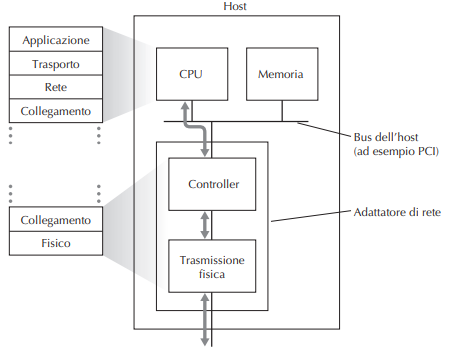
\includegraphics[width=9cm]{images/adattatore-rete.PNG}
    \caption{Adattatore di rete}
    \label{fig:adattatore-rete}
\end{figure}

Per un dato collegamento, il protocollo del livello di collegamento è sostanzialmente realizzato da un adattatore di rete (network adapter), noto anche come scheda di rete (NIC, network interface card). Il cuore della scheda di rete è il controller a livello di collegamento (link layer controller), che è di solito un chip dedicato, che implementa molti dei servizi a livello di collegamento (framing, accesso al collegamento, rilevazione degli errori). La maggior parte, quindi, delle funzionalità del controller è implementata in hardware. Fino agli anni ’90, molti adattatori di rete erano su schede fisicamente separate ma ora sono sempre più spesso integrati sulla scheda madre del calcolatore.

Lato mittente, il controller prende un datagramma, creato e memorizzato nella memoria dell’host dai livelli più alti della pila di protocolli, lo incapsula in un frame a
livello di collegamento riempiendone i vari campi dell’intestazione, e lo trasmette sul
canale di comunicazione, seguendo il protocollo di accesso al canale. Dall’altro lato,
un controller riceve l’intero frame, estrae il datagramma e lo consegna al livello di
rete. Se il protocollo del livello di collegamento fornisce il servizio di rilevazione degli errori, allora è il controller trasmittente a impostare i bit di rilevazione degli errori ed è quello ricevente che esegue il controllo. 

Lato ricevente, il software del livello di collegamento risponde agli interrupt del controller (per esempio, dovuti alla ricezione di uno o più frame), effettua la gestione di condizioni di errore e il passaggio del datagramma fino al livello di rete. Il livello di collegamento, quindi, è una combinazione di hardware e software: il luogo dove, nella pila di protocolli, il software incontra l’hardware.

\subsection{Tecniche di rilevazione e correzione degli errori}
\begin{Example}{Scenario di rilevazione e correzione degli errori}{}
    \textit{Nello scenario di riferimento, al nodo trasmittente, ai dati D che devono essere protetti da errori vengono aggiunti dei bit detti EDC (error detection and correction).}

    \begin{minipage}{\textwidth}
        \centering
        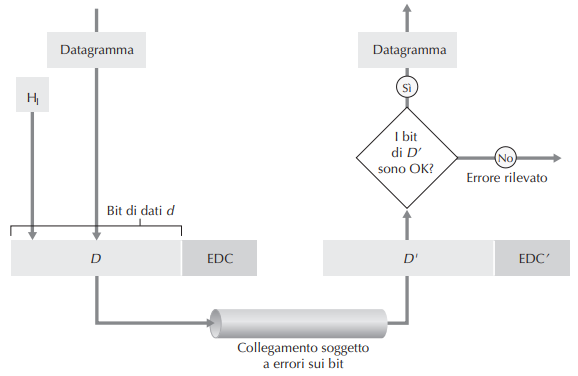
\includegraphics[width=0.7\textwidth]{images/scenario-errori.PNG}
        %\captionof{figure}{Percorso a costo minimo e tabella di inoltro per il nodo $u$}
    \end{minipage}
            
    Generalmente, i dati che devono essere protetti non includono soltanto datagrammi trasferiti verso il basso dal livello di rete per la trasmissione, ma anche le informazioni relative agli indirizzi del livello di collegamento, i numeri di sequenza e altri campi nell’intestazione del frame. I dati D e i bit EDC sono inviati in un frame al nodo ricevente. Questo legge una sequenza di bit D' ed EDC' che può essere diversa dall’originale, come risultato della modifica dei bit in transito. Il nodo ricevente deve determinare se D’ coincida con D, potendo contare soltanto su D' e su EDC'. 
\end{Example}

Le attuali tecniche non sempre consentono al nodo ricevente di rilevare se si sono verificati errori nei bit. Anche con l’utilizzo dei bit di rilevazione degli errori è possibile che ci siano degli errori non rilevati; vale a dire che il nodo ricevente potrebbe non accorgersi che le informazioni ricevute contengono errori. Di conseguenza, il ricevente potrebbe consegnare un datagramma errato al livello di rete o ignorare che il contenuto di alcuni campi nell’intestazione del frame sia stato alterato.

Dovremo quindi optare per uno schema per la rilevazione degli errori che riduca la probabilità di questo evento. Generalmente, le tecniche più sofisticate comportano un’elevata ridondanza, nel senso che sono necessari calcoli più complessi e la  trasmissione di molti bit aggiuntivi.

\subsubsection{Controllo di parità}
La forma più semplice di rilevamento degli errori è quella che utilizza un unico bit
di parità (parity bit). Supponiamo che le informazioni da inviare siano costituite da $d$ bit. In uno schema di parità pari, il mittente include un bit addizionale e sceglie il suo valore in modo da rendere pari il numero totale di bit 1 nei $d + 1$ bit trasmessi (l’informazione originale più il bit di parità). Nello schema di parità dispari, il valore del bit di parità è scelto in modo che ci sia un numero dispari di bit 1.

\begin{Example}{Parità pari a un bit}{}
    \textit{La figura mostra uno schema di parità pari, con un bit di parità inserito in un campo separato.}

    \begin{minipage}{\textwidth}
        \centering
        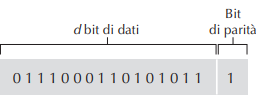
\includegraphics[width=0.4\textwidth]{images/parita-bit.PNG}
        %\captionof{figure}{Percorso a costo minimo e tabella di inoltro per il nodo $u$}
    \end{minipage}

     Con un solo bit di parità ciò che il ricevente deve fare è molto semplice: contare il numero di bit a 1 tra quelli ricevuti. Se trova un numero dispari di bit 1, sa che si è verificato almeno un errore in un bit (più precisamente, sa che si è verificato un numero dispari di errori nei bit). Tuttavia che cosa accade se si è verificato un numero pari di errori nei bit? In questo caso ci troveremmo in presenza di un errore non rilevato. Se la probabilità di errori nei bit è bassa e si può assumere che gli errori siano indipendenti, l’eventualità di errori multipli in un pacchetto è estremamente ridotta e un solo bit di parità potrebbe risultare sufficiente. Tuttavia, è stato statisticamente rilevato che gli errori tendono generalmente a verificarsi a raffiche (burst) piuttosto che in modo indipendente. La probabilità che non vengano rilevati errori a burst in un frame protetto da un solo bit di parità può avvicinarsi al 50\%. E' evidente che occorre adottare una strategia più efficiente per la rilevazione degli errori.
\end{Example}

\begin{Example}{Parità pari bidimensionale}{}
    \textit{La figura illustra una generalizzazione bidimensionale dello schema di parità con un bit.}

    \begin{minipage}{\textwidth}
        \centering
        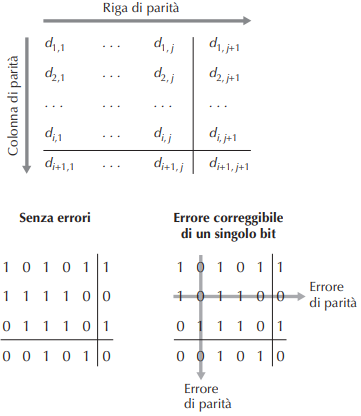
\includegraphics[width=0.5\textwidth]{images/parita-bidimensionale.PNG}
        %\captionof{figure}{Percorso a costo minimo e tabella di inoltro per il nodo $u$}
    \end{minipage}


    In questo caso, i $d$ bit del dato D sono suddivisi in $i$ righe e $j$ colonne per ognuna delle quali è stato calcolato un valore di parità. I risultanti $i + j + 1$ bit di parità contengono bit per la rilevazione dell’errore nei frame a livello di collegamento. Supponiamo ora che si verifichi un solo errore nei $d$ bit originali. Con questo schema di parità bidimensionale i bit di parità della colonna e della riga contenenti il bit errato individueranno l’errore. Il ricevente può quindi non solo rilevare che si è verificato un errore, ma può utilizzare gli indici di colonna e di riga per identificare il bit alterato e correggerlo. 
    
    La figura mostra un esempio in cui il bit a 1 in posizione $(2,2)$ è “corrotto” ed è diventato 0 (errore rilevabile e correggibile dal ricevente). Nonostante la nostra esposizione sia stata centrata sui $d$ bit originali, anche un errore negli stessi bit di parità è rilevabile e correggibile. Questo schema può rilevare (ma non correggere) qualsiasi combinazione di due errori in un pacchetto.
\end{Example}

\section{Protocolli di accesso multiplo}
Nell’introduzione di questo capitolo abbiamo osservato che esistono due tipi di collegamento di rete: punto a punto e broadcast. Il collegamento punto a punto è costituito da un trasmittente a un’estremità del collegamento e da un unico ricevente all’altra. Molti protocolli del livello di collegamento sono stati progettati per questi collegamenti, tra cui PPP (point-to-point protocol) e HDLC (high-level data link control). Il collegamento broadcast può avere più nodi trasmittenti e riceventi connessi allo stesso canale broadcast condiviso. Il termine broadcast indica che, quando un nodo trasmette un frame, il canale lo diffonde e tutti gli altri nodi ne ricevono una copia. Ethernet e Wireless LAN sono esempi di tecnologie con collegamenti broadcast.

Ipotizziamo una festa dove molte persone sono in una stanza (l’aria fornisce il canale broadcast) parlando e ascoltandosi a vicenda. Una seconda analogia è quella di una
classe nella quale insegnante e studenti condividono lo stesso singolo canale broadcast. Il problema principale in entrambi gli scenari descritti è determinare chi e quando debba parlare (cioè trasmettere). I protocolli impiegati sono estremamente vari.

Ecco qualche esempio: “Concedi a ciascuno la possibilità di parlare”; “Non parlare finché non sei interrogato”; “Non monopolizzare la conversazione”; “Alza la mano se devi porre una domanda”; “Non interrompere se qualcuno sta parlando”; “Non addormentarti quando qualcuno parla”.

Analogamente, le reti di calcolatori usano protocolli simili – i cosiddetti protocolli di
accesso multiplo – che fissano le modalità con cui i nodi regolano le loro trasmissioni
sul canale condiviso. I protocolli di accesso multiplo sono richiesti in un’ampia varietà di configurazioni di rete, comprese le LAN cablate, quelle wireless e le reti satellitari. Anche se, tecnicamente, ciascun nodo accede al canale broadcast attraverso la propria scheda di rete, in questo paragrafo useremo il termine nodo per indicare il dispositivo che trasmette e riceve. In pratica, centinaia o anche migliaia di nodi possono comunicare direttamente su un canale broadcast.

\begin{figure}[ht]
    \centering
    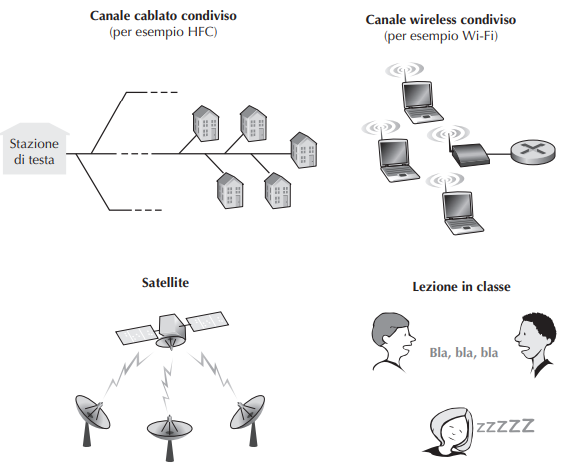
\includegraphics[width=11cm]{images/canali-accesso-multiplo.PNG}
    \caption{Canali ad accesso multiplo}
    \label{fig:canali-accesso-multiplo}
\end{figure}

Dato che tutti i nodi sono in grado di trasmettere frame, è possibile che due o più lo facciano nello stesso istante, per cui tutti i nodi riceveranno contemporaneamente più frame. Tra questi si genera una collisione a causa della quale nessuno dei nodi riceventi riuscirà a interpretare i frame che, in un certo senso, risultano ingarbugliati tra loro. Di conseguenza con la collisione si verifica una perdita di frame, mentre il canale rimane inutilizzato. E' chiaro che, se una situazione di questo genere dovesse ripetersi con eccessiva frequenza, gran parte della banda del canale risulterebbe sprecata. Per far sì che il canale broadcast venga utilizzato in modo efficiente, occorre coordinare le trasmissioni dei nodi attivi. 

Concludiamo questa panoramica rilevando che, idealmente, un protocollo di accesso multiplo per un canale broadcast con velocità di $R$ bit al secondo dovrebbe avere le
seguenti caratteristiche:
\begin{enumerate}
    \item Quando un solo nodo deve inviare dati, questo dispone di un throughput pari a $R$ bps.
    \item Quando $M$ nodi devono inviare dati, questi dispongono di un throughput pari a $R/M$ bps. Ciò non implica necessariamente che ciascuno degli $M$ nodi abbia sempre una velocità istantanea di trasmissione di $R/M$, ma che ciascun nodo dovrebbe avere una velocità di trasmissione media di $R/M$ in un dato, appropriato intervallo di tempo.
    \item Il protocollo è decentralizzato; in altre parole, non ci sono nodi principali che qualora non funzionassero correttamente potrebbero rendere inattivo l’intero sistema.
    \item Il protocollo è semplice, in modo che risulti economico da implementare.
\end{enumerate}

In generale possiamo classificare praticamente tutti i protocolli di accesso multiplo in una di queste categorie: protocolli a suddivisione del canale (channel partitioning protocol), protocolli ad accesso casuale (random access protocol) e protocolli a rotazione (taking-turn protocol).

\begin{figure}[ht]
    \centering
    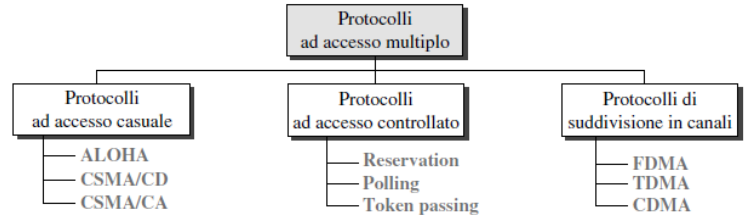
\includegraphics[width=11cm]{images/protocolli-mac.PNG}
    \caption{Tassonomia dei protocolli ad accesso multiplo}
    \label{fig:protocolli-mac}
\end{figure}

\subsection{Protocolli a suddivisione del canale}
Il multiplexing a divisione di tempo, TDM (time division multiplexing) e quello a divisione di frequenza, FDM (frequency division multiplexing), sono due tecniche che possono essere utilizzate per suddividere la larghezza di banda di un canale broadcast fra i nodi che lo condividono. Per esempio, supponiamo che il canale supporti $N$ nodi e che la sua velocità di trasmissione sia di $R$ bps. TDM suddivide il tempo in intervalli di tempo (time frame) e poi divide ciascun intervallo di tempo in $N$ slot temporali (time slot). Si noti che il time frame di TDM non deve essere confuso con l’unità di dati a livello di collegamento che le schede di rete si scambiano, che è anch’essa chiamata frame. Per ridurre la confusione, in questo paragrafo ci riferiremo all’unità di dati del livello di collegamento come a un pacchetto. Ogni slot è quindi assegnato a uno degli $N$ nodi. Ogni volta che un nodo ha un pacchetto da inviare, trasmette i bit del pacchetto durante lo slot di tempo assegnatogli. Generalmente, le dimensioni dello slot sono stabilite in modo da consentire la trasmissione di un singolo pacchetto. 

Ritornando alla nostra analogia con la festa, se questa è regolata da TDM, consente a un invitato di parlare per un intervallo di tempo stabilito. Lo stesso tempo spetterà quindi a un altro invitato, e così via. Una volta che tutti hanno avuto l’opportunità di parlare, la sequenza si ripete.

TDM viene utilizzato in quanto riesce a evitare le collisioni ed è perfettamente imparziale: ciascun nodo ottiene, durante ciascun intervallo di tempo, un tasso trasmissivo di $R/N$ bps. In ogni caso, TDM presenta due specifici inconvenienti. In effetti anche quando non vi sono altri nodi che devono inviare un pacchetto, quello che vuole trasmettere è vincolato ad attendere il suo turno nella sequenza di trasmissione e a non superare il limite medio di $R/N$ bps. Immaginiamo che ci sia un solo invitato che abbia qualcosa da dire e che questa sia una delle rare circostanze in cui tutti vogliano ascoltare. In questo particolare caso, è evidente che TDM risulta una pessima scelta di protocollo per l’accesso multiplo in questa particolare festa. 

Mentre TDM suddivide il canale condiviso in intervalli di tempo, FDM lo divide in frequenze differenti (ciascuna con una larghezza di banda di $R/N$) e assegna ciascuna frequenza a un nodo. Quindi, a partire da un canale da $R$ bps, FDM crea $N$ canali di $R/N$ bps. FDM condivide alcuni vantaggi e alcuni svantaggi del precedente protocollo. Anche FDM evita le collisioni e divide equamente la larghezza di banda tra gli $N$ nodi. Tuttavia, anche con FDM la larghezza di banda è limitata a $R/N$, pure quando vi è un solo nodo che ha un pacchetto da spedire.

\begin{figure}[ht]
    \centering
    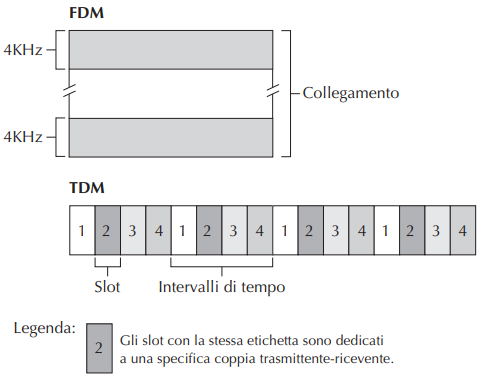
\includegraphics[width=8cm]{images/tdm-fdm.PNG}
    \caption{Esempi di TDM e FDM con quattro nodi}
    \label{fig:tdm-fdm}
\end{figure}

\subsection{Protocolli ad accesso casuale}
Nell'accesso casuale (random access) nessuna stazione è superiore alle altre e nessuna ha il controllo sulle altre. Ogni volta che una stazione ha dei dati da inviare, usa una procedura definita dal protocollo per decidere se spedire o se attendere. Tale decisione dipende dallo stato del mezzo trasmissivo (inattivo o occupato). In altre parole, ogni stazione può trasmettere quando vuole, a condizione che segua la procedura predefinita, compreso il test sullo stato del mezzo trasmissivo.

Due caratteristiche danno il nome a questo metodo. Primo, non c'è un tempo programmato nel quale la stazione deve trasmettere, la trasmissione tra le stazioni è casuale. Ecco perché questi metodi vengono chiamati ad accesso casuale. Secondo, nessuna regola specifica quale sarà la prossima stazione a trasmettere. Esse competono una con l'altra per accedere al mezzo trasmissivo. Ecco perché questi metodi sono anche chiamati di contesa (le stazioni si contendono il mezzo trasmissivo).

Nei protocolli ad accesso casuale ogni stazione ha il diritto di accedere al mezzo senza essere controllata da nessun altra stazione. Tuttavia, se più di una stazione cerca di trasmettere in contemporanea, avviene un conflitto d'accesso, una collisione, e i frame trasmessi vengono distrutti o modificati. Per evitare il conflitto d'accesso, o per risolverlo quando avviene, ogni stazione segue una procedura basata sulle seguenti domande: quando la stazione può accedere al mezzo? Cosa può fare la stazione se il mezzo trasmissivo è occupato? Come può la stazione determinare il successo o il fallimento della trasmissione? Cosa può fare la stazione nel caso in cui ci sia stato un conflitto d'accesso?

\subsubsection{ALOHA}
ALOHA, il primo metodo ad accesso casuale, è stato sviluppato all'Università delle Hawaii nei primi anni 70. E' stato ideato per l'uso in una LAN radio (wireless) ma può essere utilizzato su qualsiasi mezzo condiviso.

Dato che il mezzo trasmissivo è condiviso tra tutte le stazioni, è ovvio che ci possono essere delle collisioni. Quando una stazione invia dei dati, un'altra può tentare di fare la stessa cosa contemporaneamente. In questo caso avviene una collisione e i dati trasmessi sono alterati.

\subsubsection{ALOHA puro}
La versione originale del protocollo ALOHA viene chiamata ALOHA puro. E' un protocollo semplice ed elegante. L'idea è che ogni stazione può inviare un frame tutte le volte che ha qualcosa da inviare (accesso multiplo). Tuttavia, siccome il canale da condividere con le altre stazioni è unico, possono avvenire collisioni tra i frame delle diverse stazioni. 

\begin{Example}{ALOHA puro}{}
    \textit{Nell'esempio ci sono quattro stazioni che si contendono l'accesso al canale condiviso. La figura mostra che ogni stazione invia due frame, quindi in totale nel mezzo condiviso ce ne sono otto. Alcuni dei frame collidono a causa della contesa per il canale condiviso.}
    
    \begin{minipage}{\textwidth}
        \centering
        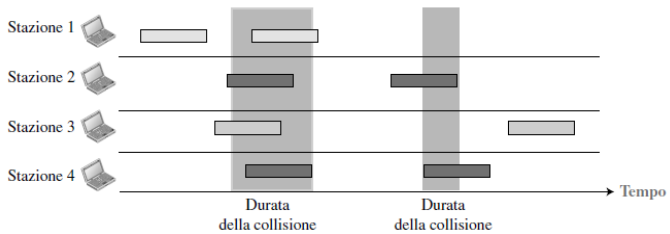
\includegraphics[width=0.7\textwidth]{images/aloha-puro.PNG}
        %\captionof{figure}{Percorso a costo minimo e tabella di inoltro per il nodo $u$}
    \end{minipage}

     La figura mostra che solo due frame sopravvivono: uno della stazione 1 e uno della stazione 3. E' bene notare che è sufficiente che due frame collidano anche solo per un singolo bit per portare alla distruzione entrambi i frame, nella loro totalità. In caso di collisione è necessario inviare nuovamente tutti i frame che sono stati distrutti durante la trasmissione.
\end{Example}

Il protocollo ALOHA si basa sull'invio di un riscontro da parte del ricevente. Quando una stazione invia un frame, si aspetta che il ricevente invii un riscontro. Se esso non arriva dopo un certo periodo di tempo (timeout), la stazione assume che il frame (o il riscontro) siano andati distrutti e reagisce trasmettendo nuovamente il frame.

Una collisione coinvolge due o più stazioni. Se tutte queste stazioni tentano di reinviare i loro frame subito dopo il timeout, avverrà immediatamente una nuova collisione. Secondo le specifiche del protocollo ALOHA puro quando il periodo di timeout è trascorso, ogni stazione aspetta un ulteriore periodo di tempo di durata casuale prima di trasmettere nuovamente il suo frame. La casualità aiuterà ad evitare altre collisioni. Questo lasso di tempo viene chiamato tempo di back-off (back-off time) $T_B$.

L'ALOHA puro prevede un secondo metodo per evitare che i frame ritrasmessi congestionino il canale. Dopo un numero massimo di tentativi di ritrasmissione $K_{\max}$, una stazione deve interrompere i suoi tentativi e provare solamente più tardi.

Il periodo di timeout equivale al massimo ritardo di propagazione di un round-trip (andata e ritorno) tra le stazioni. Quindi è due volte la quantità di tempo necessaria per inviare un frame tra le due stazioni più lontane ($2\times T_p$). Il tempo di back-off $T_B$, è un valore scelto casualmente che normalmente dipende da $K$ (il numero di trasmissioni tentate senza successo). La formula usata per determinare $T_B$ dipende dalla specifica implementazione. Una formula comune è il back-off esponenziale binario (binary exponential back-off). In questo approccio, ad ogni ritrasmissione, per trovare $T_B$, un moltiplicatore $R$, compreso tra 0 e $(2^K-1)$, viene scelto in modo casuale e moltiplicato per $T_p$ (il tempo massimo di propagazione) o per $T_{fr}$, (il tempo medio richiesto per inviare un frame). Con questa procedura l'intervallo in cui scegliere il numero casuale aumenta di dimensione dopo ogni collisione. Il valore di $K_{\max}$ normalmente scelto è 15.

\begin{Example}{Calcolo back-off}{}
    \textit{Le stazioni in una rete wireless ALOHA sono a una distanza massima di 600 km.} 
    
    Supponendo che i segnali si propaghino a $3\times 10$ m/s, troviamo:
    \begin{equation*}
        T_p = (600\times 10^3)/(3\times 10^8) = 2\textit{ ms}
    \end{equation*}
    Per $K=2$ l'intervallo di $R$ è $\{0, 1, 2, 3\}$. Ciò significa che $T_B$ può essere 0, 2, 4 o 6 ms, sulla base del risultato della variabile casuale $R$.
\end{Example}

Vediamo ora la lunghezza dell'intervallo, chiamato tempo di vulnerabilità, durante il quale c'è la possibilità che avvengano collisioni. Supponiamo che le stazioni inviino dei frame di lunghezza fissa con ogni frame che impiega $T_{fr}$ secondi per essere inviato.

\begin{figure}[ht]
    \centering
    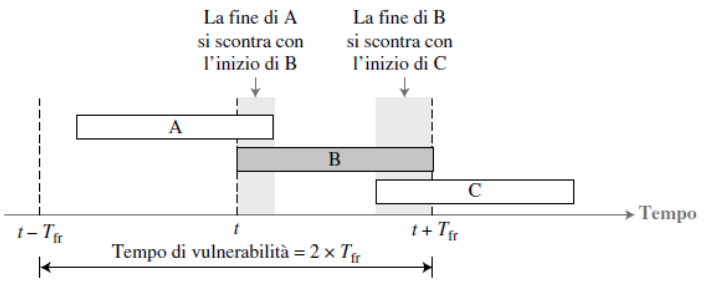
\includegraphics[width=8cm]{images/tempo-vulnerabilità.PNG}
    \caption{Tempo di vulnerabilità nel protocollo ALOHA puro}
    \label{fig:tempo-vulnerabilità}
\end{figure}

La stazione $B$ inizia ad inviare un frame al tempo $t$. Ora, immaginiamo che la stazione $A$ abbia iniziato ad inviare il suo frame dopo $t - T_{fr}$. Ciò porta a una collisione tra i frame della stazione $B$ e quelli della stazione $A$. Inoltre, supponiamo che la stazione $C$ inizi ad inviare un frame prima del tempo $t + T_{fr}$. Anche in questo caso ci sarà una collisione tra i frame della stazione $B$ e quelli della stazione $C$.

Guardando la Figura \ref{fig:tempo-vulnerabilità} vediamo che il tempo di vulnerabilità, durante il quale in ALOHA puro potrebbe avvenire una collisione, è 2 volte il tempo di trasmissione del frame ($2\times T_{fr}$).

Chiamiamo $G$ il numero medio di frame generati dal sistema durante il tempo di trasmissione di un frame. Si può dimostrare che il numero medio di frame trasmessi con successo per ALOHA puro è $S = G\times e^{- 2G}$. Il throughput massimo $S_{\max}$ è di 0,184, per $G = 1/2$. Questo valore può essere ricavato impostando a 0 la derivata di $S$ rispetto a $G$. In altre parole, se metà di un frame viene generata durante il terapo di trasmissione di uno (un frame dura il tempo di trasmissione di due), allora il 18,4\% di tali frame raggiunge la destinazione con successo. Ci si aspetta che $G = 1/2$ produca il throughput massimo in quanto il tempo di vulnerabilità è pari a 2 volte il tempo di trasmissione di un frame.

Quindi, se una stazione genera solo un frame nel suo tempo di vulnerabilità (e nessun altra stazione ne genera uno in quel tempo), esso raggiungerà la sua destinazione con successo.

L’efficienza di un protocollo di accesso multiplo che fa uso di slot temporali è definita come la frazione di slot riusciti in presenza di un elevato numero di nodi attivi che hanno sempre un elevato numero di pacchetti da spedire. Notiamo che se non venisse utilizzata alcuna forma di controllo dell’accesso e se ciascun nodo ritrasmettesse subito dopo che si è effettuata la
collisione, l’efficienza sarebbe zero. 

Se un frame va in collisione, allora il nodo lo ritrasmette immediatamente (dopo aver completato la trasmissione del frame) con probabilità $p$. Altrimenti, attenderà il tempo di trasmissione del frame. Trascorso questo tempo, il nodo ritrasmetterà il frame con probabilità $p$ o aspetterà, restando inattivo per un altro periodo di tempo, con probabilità $1 – p$. Per determinare l’efficienza massima di ALOHA puro, analizziamo un singolo nodo. A ogni dato istante, la probabilità che un nodo stia trasmettendo è $p$. Supponiamo che la trasmissione di un frame inizi al tempo $t_0$. Affinché questo frame sia trasmesso con esito positivo nessun altro nodo può cominciare la sua trasmissione nell’intervallo di tempo $(t_0 – 1, t_0]$, in quanto si sovrapporrebbe con l’inizio della trasmissione del frame del nodo $i$. La probabilità che tutti gli altri nodi non diano inizio a una trasmissione in questo intervallo è $(1 – p)^{N –1}$. Analogamente, nessun altro nodo può iniziare la trasmissione mentre il nodo $i$ sta trasmettendo, in quanto si sovrapporrebbe all’ultima parte della trasmissione di quel frame. La probabilità che tutti gli altri nodi non comincino a trasmettere in questo intervallo è anch’essa $(1 – p)^{N –1}$. Di conseguenza, possiamo notare che la probabilità che un certo nodo abbia successo nella trasmissione è $p(1 – p)^{2(N –1)}$. Ricavando il limite per $N$ che tende all’infinito, otteniamo che l’efficienza massima del protocollo ALOHA puro è solo $1/(2e)=0,18$. Questo è il prezzo che il protocollo ALOHA deve pagare per la completa decentralizzazione.

\subsubsection{Slotted ALOHA}
Lo Slotted ALOHA è stato inventato per migliorare l'efficienza dell'ALOHA puro. Nello Slotted ALOHA il tempo viene diviso in slot (intervalli di dimensione fissa) di $T_{fr}$ secondi e le stazioni vengono forzate a trasmettere solo all'inizio degli slot.

Siccome le stazioni sono sincronizzate e possono trasmettere solo all'inizio degli slot, se si lasciano sfuggire tale momento, devono attendere fino all'inizio dello slot successivo. Ciò significa che, a questo punto, la stazione che ha avviato la trasmissione nello slot precedente avrà ormai già finito di inviare il suo frame. Naturalmente c'è ancora la possibilità di collisione se due stazioni cercano di trasmettere all'inizio dello stesso slot.
I nodi devono essere d'accordo nel confine fra gli intervalli, e ciò può essere fatto facendo emettere da una attrezzatura speciale un breve segnale all'inizio di ogni intervallo.

Nella nostra descrizione assumeremo che: tutti i frame consistano esattamente di $L$ bit; il tempo sia suddiviso in slot di $L/R$ secondi (cioè che uno slot equivalga al tempo di trasmissione di un pacchetto); i nodi comincino la trasmissione dei frame solo all’inizio degli slot; i nodi siano sincronizzati in modo che tutti sappiano quando iniziano gli slot; qualora in uno slot due o più frame collidano, tutti i nodi della rete rilevino l’evento prima del termine dello slot. Indichiamo con $p$ una probabilità, vale a dire un numero tra 0 e 1. Le operazioni dei nodi slotted ALOHA sono semplici.
\begin{itemize}
    \item Quando un nodo ha un nuovo frame da spedire, attende fino all’inizio dello slot successivo e poi trasmette l’intero frame.
    \item Se non si verifica una collisione, l’operazione ha avuto successo, quindi non occorre effettuare una ritrasmissione e il nodo può predisporre l’invio di un nuovo frame.
    \item Se si verifica una collisione, il nodo la rileva prima del termine dello slot e ritrasmette con probabilità $p$ il suo frame durante gli slot successivi, fino a quando l’operazione non ha successo.
\end{itemize}

Questo protocollo sembra possedere grandi vantaggi. A differenza della suddivisione del canale, slotted ALOHA consente a un singolo nodo di trasmettere continuamente pacchetti alla massima velocità del canale, quando è il solo nodo attivo. Un nodo si dice attivo se ha un frame da trasmettere. Slotted ALOHA è anche fortemente decentralizzato, in quanto ciascun nodo rileva le collisioni e decide indipendentemente quando ritrasmettere, anche se è comunque necessario che gli slot siano sincronizzati ai nodi. Slotted ALOHA funziona bene quando è attivo un solo nodo, ma è altrettanto efficiente in presenza di molti nodi attivi? Esistono in questo caso due possibili problemi. In primo luogo, una certa frazione degli slot presenterà collisioni e di conseguenza andrà “sprecata”. Il secondo problema è che una grande frazione degli slot risulterà vuota, perché tutti i nodi attivi terminano la trasmissione in conseguenza della politica di trasmissione probabilistica. I soli slot non sprecati saranno esattamente quelli utilizzati da un solo nodo per trasmettere.

Supponiamo che ciascun nodo abbia sempre un frame da spedire e che il nodo trasmetta con probabilità $p$ un nuovo frame o uno che ha già subito una collisione. In primo luogo, ipotizziamo di avere $N$ nodi. In questo caso la probabilità che un dato slot sia vincente è data dalla probabilità che un solo nodo trasmetta, mentre i rimanenti $N – 1$ rimangono inattivi. La probabilità che un dato nodo trasmetta è $p$; la probabilità che i rimanenti nodi non trasmettano è $(1 – p)^{N–1}$. Quindi la probabilità di successo di un dato nodo è $p(1 – p)^{N –1}$. Poiché ci sono $N$ nodi, la probabilità che un nodo arbitrario abbia successo è $Np(1 – p)^{N –1}$. Di conseguenza, con $N$ nodi attivi, l’efficienza dello slotted ALOHA è $Np(1 – p)^{N–1}$. Per ottenere la massima efficienza con $N$ nodi attivi bisogna trovare il valore $p^*$ che massimizza questa espressione. Per ottenere la massima efficienza per un elevato numero di nodi attivi, ricaviamo il limite di $Np^* (1 – p^*)^{N –1}$ per $N$ che tende all’infinito. Dopo aver svolto questi calcoli, otterremo che l’efficienza massima del protocollo è data da $1/e = 0,37$. Vale a dire che quando un gran numero di nodi ha molti pacchetti da trasmettere, allora (nel caso migliore) solo il 37\% degli slot compie lavoro utile. Quindi, l’effettiva velocità di trasmissione del canale non è $R$ bps, ma soltanto $0,37 R$ bps!

\subsubsection{CSMA: accesso multiplo con rilevamento della portante}
Nei due protocolli ALOHA i nodi prendono la decisione di trasmettere indipendentemente dall’attività degli altri nodi collegati al canale broadcast. In particolare, un nodo non presta attenzione al fatto che vi sia un altro nodo che sta trasmettendo né arresta la trasmissione se un altro nodo inizia a interferire con la sua trasmissione. Nella nostra analogia con il comportamento umano, i protocolli ALOHA corrispondono a un maleducato che continua a parlare senza preoccuparsi del fatto che altri stiano conversando tra loro.

Disponiamo di “protocolli” che ci consentono non solo di comportarci più educatamente, ma anche di diminuire il tempo di “collisione” tra le diverse conversazioni e, di conseguenza, di aumentare la quantità di dati che viene scambiata. In particolare, esistono due regole importanti per dialogare in modo civile, che sono le seguenti. 
\begin{itemize}
    \item Ascoltare prima di parlare. Se qualcun altro sta parlando, aspettare finché abbia concluso. Nel mondo delle reti, ciò è chiamato rilevamento della portante (carrier sensing): un nodo ascolta il canale prima di trasmettere. Se il canale sta già trasmettendo un frame, il nodo aspetta finché rileva che il canale è libero per un intervallo di tempo e quindi inizia la trasmissione. 
    \item Se qualcun altro comincia a parlare insieme a voi, smettete di parlare. Nel mondo delle reti, ciò si chiama rilevamento della collisione (collision detection): il nodo che sta trasmettendo rimane contemporaneamente in ascolto del canale. Se osserva che un altro nodo sta trasmettendo un frame che interferisce col suo, arresta la propria trasmissione, aspetta un intervallo di tempo casuale e poi ripete il processo.
\end{itemize}

Queste due regole sono alla base dei protocolli CSMA (carrier sense multiple access, accesso multiplo con rilevamento della portante).

La prima domanda è: perché, se tutti i nodi eseguono il rilevamento della portante,
si verificano collisioni? Dopo tutto, i nodi rinunciano alla trasmissione quando rilevano che qualcun altro sta trasmettendo. La risposta alla domanda può essere meglio
spiegata mediante diagrammi spazio-temporali. 

\begin{Example}{Diagramma spazio-temporale CSMA con trasmissioni in collisione}{}
    \textit{La figura ne illustra uno relativo a quattro nodi (A, B, C, D). L’asse orizzontale mostra la posizione dei nodi sul canale condiviso e quello verticale rappresenta il tempo.}

    \begin{minipage}{\textwidth}
        \centering
        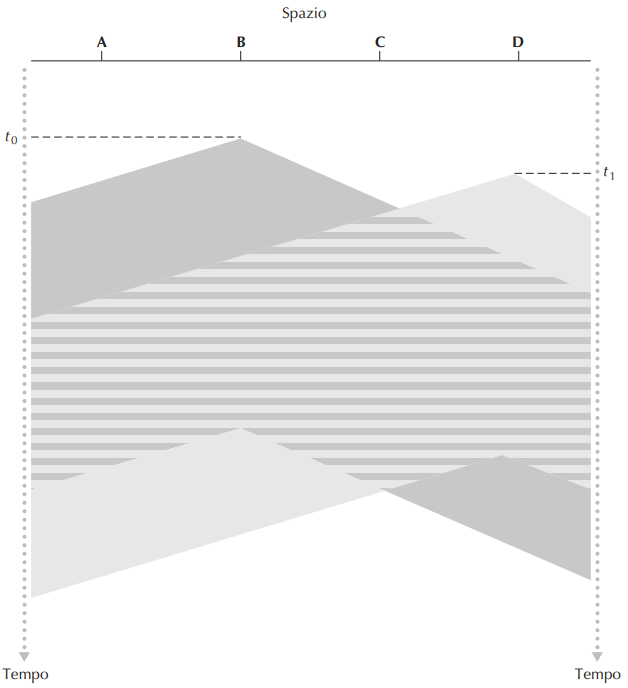
\includegraphics[width=0.5\textwidth]{images/diagramma-temporale-csma.PNG}
        %\captionof{figure}{Percorso a costo minimo e tabella di inoltro per il nodo $u$}
    \end{minipage}

    All’istante $t_0$, il nodo B rileva che il canale è inattivo (nessun altro nodo sta trasmettendo), comincia la trasmissione e i suoi bit si propagano in entrambe le direzioni lungo il mezzo trasmissivo. La propagazione verso valle dei bit di B al crescere del tempo indica che è necessario un intervallo di tempo non nullo per l’effettiva propagazione dei bit di B lungo il canale (benché questa avvenga a una velocità paragonabile a quella della luce). Al tempo $t_1 > t_0$, il nodo D ha un frame da spedire. Sebbene al tempo $t_1$ il nodo B stia ancora trasmettendo, i suoi bit non hanno ancora raggiunto D e quindi, in quell’istante, D ritiene libero il canale. Nel pieno rispetto del protocollo, D allora comincia a trasmettere il suo frame. Dopo un breve periodo, la trasmissione di B comincerà a interferire con quella di D. 

    Dalla figura risulta evidente che il ritardo di propagazione da un estremo all’altro di un canale broadcast (il tempo richiesto da un segnale per propagarsi da un nodo all’altro) avrà un ruolo cruciale nel determinare le sue prestazioni. Maggiore è questo ritardo, maggiore sarà la possibilità che il nodo, pur attento a rilevare la portante, non si accorga che è già cominciata la trasmissione da parte di un altro nodo.    
\end{Example}


Il tempo di vulnerabilità per il CSMA è pari al tempo di propagazione $T$. È il tempo necessario affinché un segnale si propaghi da un'estremità all'altra del mezzo. Quando una stazione invia un frame e un'altra cerca di inviarne un altro allo stesso tempo, avviene una collisione. Ma se il primo bit del frame raggiunge l'estremità del mezzo, ogni stazione ha già percepito il bit ed evita di trasmettere. 

Cosa deve fare una stazione se il canale è occupato? Cosa deve fare se il canale è inattivo? Sono stati ideati tre metodi per rispondere a queste domande: 1-persistente, non persistente, p-persistente.

\begin{figure}[ht]
    \centering
    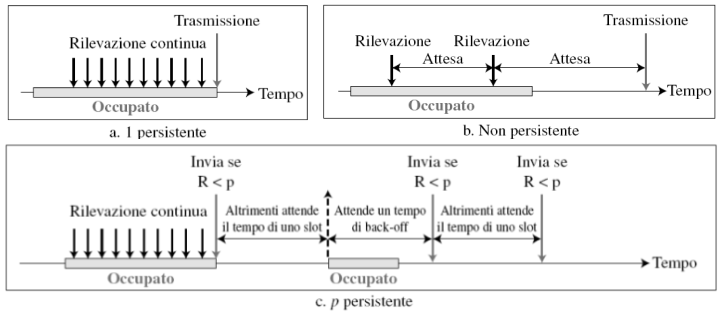
\includegraphics[width=11cm]{images/metodi-persistenza.PNG}
    \caption{Comportamento dei tre metodi di persistenza}
    \label{fig:metodi-persistenza}
\end{figure}

\begin{itemize}
    \item \textit{1 persistente.} Il metodo dell'1 persistente è semplice e chiaro. Secondo questo metodo, se una stazione trova il canale attivo continua a controllarlo fino a quando non diviene inattivo. Quando finalmente il canale diviene inattivo la stazione invia immediatamente il suo frame (con probabilità 1). Questo metodo ha la più alta probabilità di generare collisioni in quanto due o più stazioni possono trovare il mezzo trasmissivo inattivo ed inviare immediatamente i loro frame.
    \item \textit{Non persistente.} Nel metodo non persistente una stazione che deve inviare un frame rileva il mezzo trasmissivo. Se è inattivo, trasmette immediatamente. Se non è inattivo, attende un lasso di tempo casuale e poi effettua nuovamente la rilevazione. L'approccio non persistente riduce la probabilità di collisioni in quanto è improbabile che due o più stazioni attendano esattamente lo stesso lasso di tempo e cerchino di nuovo di trasmettere contemporaneamente. Tuttavia tale metodo riduce l'efficienza della rete in quanto il mezzo resta inattivo quando invece potrebbero esserci delle stazioni con dei frame in attesa di essere inviati.
    \item \textit{p persistente.} Il metodo p persistente viene utilizzato se il canale è stato suddiviso in intervalli fissi di tempo (slot) dove ciascuno slot ha una durata che è uguale o maggiore rispetto al tempo massimo di propagazione. L'approccio p persistente unisce i vantaggi delle altre due strategie. Riduce la possibilità di collisione e migliora l'efficienza. Secondo tale metodo, dopo che la stazione ha trovato il mezzo trasmissivo inattivo, segue i seguenti passi:
    \begin{enumerate}
        \item con probabilità $p$, la stazione invia il suo frame;
        \item con probabilità $q = 1-p$, la stazione attende l'inizio del prossimo slot e controlla nuovamente il mezzo trasmissivo: se il mezzo è inattivo, torna al punto 1; se è occupato, agisce come se fosse avvenuta una collisione e utilizza la procedura di back-off.
    \end{enumerate}
\end{itemize}

\subsubsection{CSMA/CD}
Il metodo CDMA non specifica la procedura da seguire a seguito di una collisione. Il Carrier Sense Multiple Access with Collision Detection (CSMA/CD) a partire dall'algoritmo CSMA aggiunge una parte relativa alla gestione delle collisioni.

In questo metodo una stazione, durante l'invio di un frame, continua a controllare il mezzo trasmissivo per verificare se la trasmissione ha avuto successo. Se è così la trasmissione è finita, in caso contrario (c'è stata una collisione) il frame dovrà essere nuovamente inviato.

\begin{Example}{Collisione nel CSMA/CD}{}
    \textit{Vediamo la figura dove due stazioni (A e C) sono coinvolte in una collisione. Entrambe le stazioni continuano a spedire i bit dei loro frame fino a quando non sono in grado di rilevare la collisione.}
    
    \begin{minipage}{\textwidth}
        \centering
        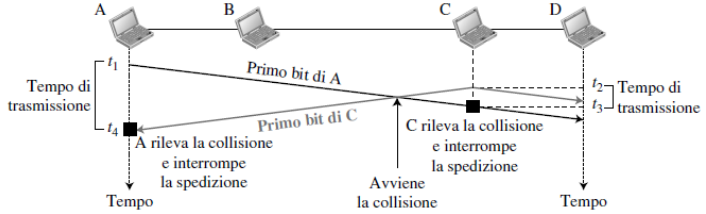
\includegraphics[width=0.7\textwidth]{images/csma_cd.PNG}
        %\captionof{figure}{Percorso a costo minimo e tabella di inoltro per il nodo $u$}
    \end{minipage}
        
    Al tempo $t_1$, la stazione A ha effettuato la sua procedura di persistenza e inizia ad inviare i bit dei suo frame. Al tempo $t_2$, la stazione C non ha ancora rilevato il primo bit inviato da A. La stazione C effettua la sua procedura di persistenza ed inizia ad inviare i bit nel suo frame, che si propagano in tutte le direzioni. La collisione avviene in un momento successivo al tempo $t_2$. La stazione C rileva una collisione al tempo $t_3$, quando riceve il primo bit del frame di A. La stazione C interrompe la trasmissione immediatamente (oppure dopo un breve lasso di tempo, ma ora si assume che sia immediatamente). La stazione A rileva la collisione al tempo $t_4$ quando riceve il primo bit del frame di C. Come reazione, anche la stazione A interrompe immediatamente la trasmissione. Guardando la figura vediamo che A trasmette per la durata di $t_4-t_1$ e C trasmette per la durata $t_3 - t_2$.
\end{Example}

Affinché il CSMA/CD possa funzionare, è necessario aggiungere un vincolo alla dimensione del frame. Prima di inviare l'ultimo bit del frame la stazione mittente deve essere in grado di rilevare una collisione, nel caso ce ne sia una, ed interrompere la trasmissione. Il motivo è che la stazione, una volta che l'intero frame è stato inviato, non ne tiene copia ed inoltre non controlla il mezzo trasmissivo per rilevare eventuali collisioni. Quindi il tempo di trasmissione del frame $T_{fr}$ deve essere almeno due volte il tempo di propagazione massimo $T_{p}$. Per comprendere la ragione, pensiamo allo scenario del caso pessimo. Se due stazioni coinvolte in una collisione si trovano alla distanza massima, il segnale dalla prima necessita del tempo $T_{p}$ per raggiungere la seconda e l'effetto della collisione necessita di un ulteriore tempo $T_{p}$ raggiungere la prima. Quindi il requisito è che la prima stazione deve essere ancora trasmissione dopo $2T_{p}$.

\begin{Example}{CSMA/CD}{}
    \textit{Una rete che utilizza il CSMA/CD ha un'ampiezza di banda di 10 Mbps. Se il tempo di propagazione massimo (compresi i ritardi nei dispositivi) è 25,6 $\mu s$, qual è la dimensione minima del frame?}

    Il tempo di trasmissione minimo del frame è $T_{fr} = 2T_{p} = 51,2\mu s$. Ciò significa, nel peggiore dei casi, che una stazione deve trasmettere per un periodo di 51,2 $\mu s$ per poter rilevare la collisione. La dimensione minima del frame è quindi $10 Mbps\times 51,2 \mu s = 512$ bit o 64 byte.
\end{Example}

Quando un solo nodo ha un frame da inviare può trasmettere alla massima velocità del canale (10 Mbps, 100 Mbps o 1 Gbps per Ethernet). Se, invece, i nodi che vogliono trasmettere sono numerosi, l’effettiva velocità di trasmissione sul canale può risultare notevolmente inferiore. Definiamo efficienza di CSMA/CD la frazione di tempo media durante la quale i frame sono trasferiti sul canale senza collisioni in presenza di un alto numero di nodi attivi, con un’elevata quantità di frame da inviare.

\subsection{Protocolli a rotazione}
Ricordiamo che due proprietà auspicabili di un protocollo di accesso multiplo sono: (1) quando un solo nodo è attivo, deve avere un throughput di $R$ bps, e (2) quando sono attivi M nodi, ciascuno deve avere un throughput vicino a $R/M$ bps. I protocolli ALOHA e CSMA possiedono la prima proprietà, ma non la seconda. Questo ha incoraggiato i ricercatori a creare un’altra classe di protocolli: i protocolli a rotazione (taking-turn protocol). Esistono decine di questi protocolli, ciascuno con molte varianti; ne vedremo qui due tra le più importanti. 

\subsubsection{Protocollo polling}
Il primo è il protocollo polling nel quale uno dei nodi, designato come principale, interpella “a turno” gli altri. In particolare, il nodo principale invia un messaggio al nodo 1, comunicandogli che può trasmettere fino a un dato numero massimo di frame. Dopo che il nodo 1 ha trasmesso dei frame, il nodo principale avvisa il nodo 2 che può iniziare a inviare un dato numero massimo di frame. Il nodo principale può determinare che un nodo ha terminato di inviare i propri frame, osservando la mancanza di segnale sul canale. La procedura prosegue in questo modo, con il nodo principale che interpella in modo ciclico tutti gli altri nodi.

Il protocollo polling elimina le collisioni e gli slot vuoti che si riscontrano nei protocolli ad accesso casuale e quindi può avere un’efficienza più elevata, ma presenta anche alcuni svantaggi. Il primo è l’introduzione del ritardo di polling: il tempo richiesto per notificare a un nodo il permesso di trasmettere. Se, per esempio, è attivo solo un nodo, allora questo trasmetterà a un tasso inferiore di R bps, in quanto il nodo principale deve contattare ciclicamente i nodi inattivi ogni volta che quello attivo ha terminato l’invio del suo numero massimo di frame. Il secondo inconveniente, potenzialmente molto più serio, è che, se il nodo principale si guasta, l’intero canale diventa inattivo.

\subsubsection{Protocollo token-passing}
Il secondo protocollo a rotazione è il protocollo token-passing (a passaggio di gettone). In questo caso non esiste un nodo principale, ma un frame, un messaggio di controllo detto token (gettone), che circola fra i nodi seguendo un ordine prefissato. Per esempio: il nodo 1 deve sempre spedire il token al nodo 2 che deve inviarlo al nodo 3 e così via fino a quando il nodo N lo restituirà al nodo 1 che riprenderà la procedura. Se il nodo che riceve il token non ha pacchetti da inviare, lo inoltra immediatamente al successivo. Altrimenti, procede a trasmettere il numero massimo di frame consentito, prima di inoltrare il token al nodo successivo. 

Questo protocollo è decentralizzato e altamente efficiente, ma non è privo di problemi. Per esempio, il guasto di un nodo può mettere fuori servizio l’intero canale. Oppure, se un nodo non riesce a inoltrare il token, occorre invocare procedure di recupero, per rimetterlo in circolazione.

\section{Indirizzamento di collegamento}
Host e router hanno indirizzi a livello di collegamento. Ciò potrebbe essere  sorprendente visto che i nodi hanno anche un indirizzo a livello di rete.  Dovreste quindi domandarvi perché abbiamo la necessità di avere indirizzi sia a livello di rete sia a livello di collegamento.

In una rete senza connessione come Internet non è possibile far sì che un datagramma raggiunga la sua destinazione solamente usando gli indirizzi IP. La ragione è che ogni datagramma in Internet, dallo stesso host sorgente allo stesso host destinazione, può prendere un percorso diverso. Gli indirizzi IP sorgente e destinazione definiscono le due estremità della rete, ma non dicono attraverso quali collegamenti deve passare il datagramma. In una rete senza connessione, è necessario avere un ulteriore meccanismo di indirizzamento: gli indirizzi di livello collegamento. Un indirizzo di livello collegamento (indirizzo di collegamento, link-layer address, link address) è spesso chiamato anche indirizzo fisico oppure indirizzo MAC (MAC address).

I collegamenti sono ovviamente controllati dal livello di collegamento e utilizzano indirizzi di questo livello. Quando un datagramma passa dal livello di rete al livello di collegamento, esso viene racchiuso all'interno di un frame e viene aggiunta un'intestazione che contiene due indirizzi di livello collegamento (sorgente e destinazione del frame). Questi due indirizzi vengono cambiati ogni volta che il frame passa da un collegamento ad un altro.

\begin{Example}{Indirizzi IP e indirizzi di livello collegamento in una piccola rete}{}
    \textit{Nella rete della figura ci sono 3 collegamenti e 2 router. Abbiamo mostrato solo 2 host: Gaia (sorgente) e Gabriele (destinazione). Per ogni host vengono indicati due indirizzi, gli indirizzi IP (N) e quelli di collegamento (L).}
    
    \begin{minipage}{\textwidth}
        \centering
        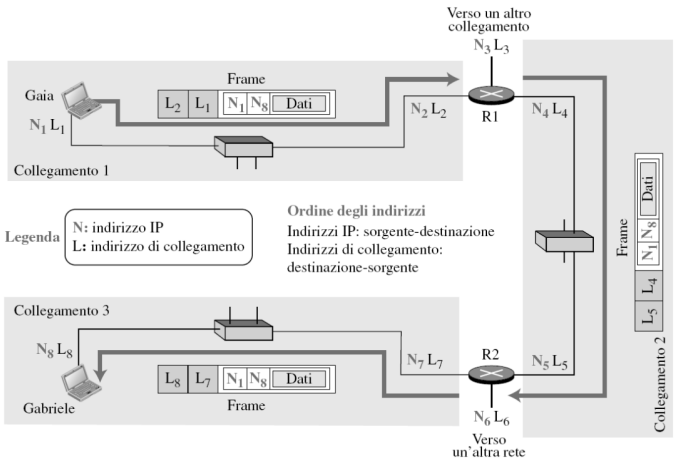
\includegraphics[width=0.7\textwidth]{images/indizirizzi-ip-mac.PNG}
        %\captionof{figure}{Percorso a costo minimo e tabella di inoltro per il nodo $u$}
    \end{minipage}
    
    Da notare che un router ha tante coppie di indirizzi quanti sono i suoi  collegamenti. In tutto abbiamo mostrato 3 frame, uno per ogni collegamento. Ogni frame trasporta lo stesso datagramma che contiene sempre gli stessi indirizzi di sorgente e destinazione (N1 e N8), ma gli indirizzi di collegamento del frame cambiano su ciascun collegamento. Nel collegamento 1, gli indirizzi di collegamento sono $L_1$ ed $L_2$. Nel collegamento 2, essi sono $L_4$ e $L_5$. Nel collegamento 3 sono $L_7$ e $L_8$. Da notare che gli indirizzi IP e gli indirizzi di collegamento non seguono lo stesso ordine. Per gli indirizzi IP, l'indirizzo sorgente viene prima di quello di destinazione; per gli indirizzi di collegamento invece l'indirizzo destinazione viene prima di quello sorgente. I datagrammi ed i frame sono stati progettati in questo modo e quindi rispettiamo questa convenzione.
\end{Example}

\subsection{Indirizzi MAC}
In realtà, non sono i nodi (cioè, gli host e i router) ad avere indirizzi a livello di collegamento, ma sono i loro adattatori (schede di rete) a possederli. Un host o un router con più interfacce di rete avrà più indirizzi a livello di collegamento associati a esse, esattamente come accadeva per gli indirizzi IP.

Gli indirizzi a livello di collegamento sono indicati con varie terminologie che vanno da indirizzo fisico, indirizzo LAN o indirizzo MAC. Poiché quest’ultimo sembra essere il termine più utilizzato, d’ora in avanti ci riferiremo a questi indirizzi come a indirizzi MAC. Per molte LAN (come Ethernet e 802.11), l’indirizzo MAC è lungo sei byte, il che consente di avere $2^{48}$ possibili indirizzi. Questi indirizzi sono generalmente espressi in notazione esadecimale, scrivendo due cifre esadecimali per ogni byte. 

Un’interessante proprietà degli indirizzi MAC è che non esistono due schede di rete con lo stesso indirizzo. Ciò può sembrare sorprendente, dato che le schede di rete sono costruite in differenti paesi da diverse società. Come può un’azienda che costruisce schede a Taiwan essere sicura di usare indirizzi diversi da una che le costruisce in Belgio? La risposta è che la IEEE sovrintende alla gestione degli indirizzi MAC. In particolare, quando una società vuole costruire schede di rete, compra un blocco di spazio di indirizzi, costituito da $2^{24}$ indirizzi, a un prezzo simbolico. IEEE riserva il blocco di $2^{24}$ indirizzi, fissando i primi 24 bit dell’indirizzo e lasciando alla società il compito di assegnare a ciascuna scheda di rete una specifica combinazione dei 24 bit rimanenti.

L’indirizzo MAC di una scheda di rete ha una struttura piatta (cioè non gerarchica)
e non cambia mai. Ricordiamo che, al contrario, gli indirizzi IP hanno una struttura gerarchica (una parte per la rete e una parte per l’host), e che l’indirizzo IP di un nodo deve essere cambiato quando l’host si sposta, cioè quando cambia la rete al quale è collegato. L’indirizzo MAC di una scheda di rete è analogo al numero di codice fiscale di una persona, che ha anch’esso struttura orizzontale e non varia a seconda del luogo in cui la persona si trasferisce. Gli indirizzi IP invece sono analoghi all’indirizzo postale di una persona. Questi indirizzi hanno una struttura gerarchica e devono essere aggiornati quando la persona cambia residenza.

\subsection{Protocollo per la risoluzione degli indirizzi (ARP)}
Dato che esistono sia indirizzi del livello di rete (come gli indirizzi IP di Internet) sia indirizzi del livello di collegamento (gli indirizzi MAC), si presenta la necessità della loro conversione. Internet affida questo compito al protocollo di risoluzione degli
indirizzi (ARP, address resolution protocol). 

\begin{Example}{ARP}{}
    \textit{Per comprendere la necessità di un protocollo come ARP, considerate la rete illustrata in figura. In questo semplice esempio, ciascun nodo ha un indirizzo IP e la scheda di ciascun nodo ha un indirizzo MAC. Come al solito, gli indirizzi IP sono rappresentati in notazione decimale puntata e gli indirizzi MAC in notazione esadecimale.}

    \begin{minipage}{\textwidth}
        \centering
        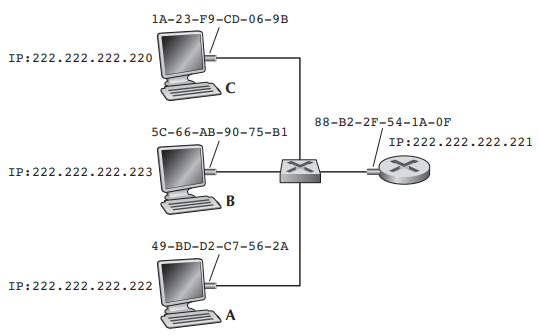
\includegraphics[width=0.5\textwidth]{images/es-arp.PNG}
        %\captionof{figure}{Percorso a costo minimo e tabella di inoltro per il nodo $u$}
    \end{minipage}

    Supponiamo ora che il nodo con l’indirizzo IP \texttt{222.222.222.220} voglia inviare un datagramma IP al nodo \texttt{222.222.222.222}. In questo esempio i nodi sorgente e destinazione appartengono alla stessa sottorete, dal punto di vista dell’indirizzamento. Per trasmettere un datagramma, il nodo trasmittente deve fornire alla sua scheda di rete non solo il datagramma IP, ma anche l’indirizzo MAC del nodo destinatario \texttt{222.222.222.222}. Quando gli vengono passati il datagramma IP e l’indirizzo MAC, la scheda del nodo trasmittente deve costruire un frame contenente l’indirizzo MAC del nodo di destinazione e immetterlo nella LAN.

    Un’importante problematica affrontata in questo paragrafo è come il nodo trasmittente riesca a determinare l’indirizzo MAC del nodo destinazione con indirizzo IP \texttt{222.222.222.222}. Come potete immaginare, bisogna utilizzare ARP. Un modulo ARP nel nodo sorgente riceve in input un indirizzo IP della stessa LAN e restituisce l’indirizzo MAC corrispondente. Nell’esempio trattato, il nodo trasmittente passa al suo modulo ARP l’indirizzo IP \texttt{222.222.222.222} e ARP gli restituisce il corrispondente indirizzo MAC, cioè \texttt{49-BD-D2-C7-56-2A}.
\end{Example}

Abbiamo quindi visto che un modulo ARP traduce un indirizzo IP in un indirizzo MAC. Ora che abbiamo visto che cosa fa ARP, cerchiamo di capire come funziona. Nella
RAM dei nodi vi è una tabella ARP che contiene la corrispondenza tra indirizzi IP
e MAC. La tabella contiene anche un valore relativo al TTL (time-to-live, tempo di vita), che indica quando bisognerà eliminare una data voce dalla tabella.

\begin{figure}[ht]
    \centering
    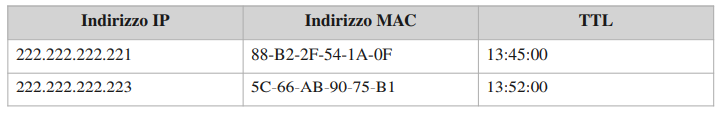
\includegraphics[width=11cm]{images/tabella-arp.PNG}
    \caption{Una possibile tabella ARP per il nodo \texttt{222.222.222.220}}
    \label{fig:tabella-arp}
\end{figure}

Notiamo che la tabella non contiene necessariamente una voce per ciascun nodo della sottorete; alcuni nodi possono essere stati cancellati (perché scaduto il loro TTL), altri possono non essere mai stati inseriti. Il tipico TTL è di 20 minuti, da quando una voce viene inserita nella tabella ARP.

Il protocollo ARP è uno dei protocolli ausiliari definiti a livello di rete. Appartiene al livello di rete, ma abbiamo deciso di rimandare la sua analisi fino ad ora proprio perché il suo scopo è associare gli indirizzi IP agli indirizzi di collegamento. L'ARP accetta in input un indirizzo IP, individua l'indirizzo di collegamento corrispondente e lo passa al livello di collegamento.

\begin{figure}[ht]
    \centering
    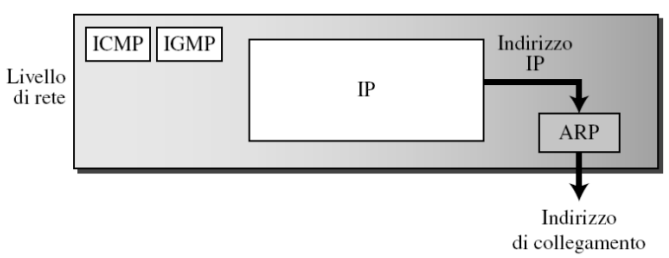
\includegraphics[width=8cm]{images/posizione-arp.PNG}
    \caption{Posizione dell'ARP nella pila TCP/IP}
    \label{fig:posizione-arp}
\end{figure}

Ogni volta che un host o un router deve trovare l'indirizzo di collegamento di un altro host o router che si trova all'interno della sua rete, invia un pacchetto di richiesta ARP che comprende l'indirizzo di collegamento, l'indirizzo IP del mittente e l'indirizzo IP del ricevente. Siccome il mittente non conosce ancora l'indirizzo di collegamento del ricevente, la richiesta viene trasmessa usando un broadcast a livello di collegamento. L'invio broadcast è ottenuto per mezzo del corrispondente indirizzo broadcast, in modo che la richiesta raggiunga tutti i nodi all'interno della rete locale.

Ogni host o router nella rete locale riceve ed elabora il pacchetto di richiesta ARP, ma solo il ricevente designato riconosce il suo indirizzo IP e restituisce un pacchetto di risposta ARP che contiene i suoi indirizzi IP e di collegamento. Il pacchetto di risposta viene inviato in modalità unicast direttamente al nodo che ha inviato la richiesta.

\begin{Example}{Protocollo ARP nella stessa sottorete}{}
    \textit{Nella figura, il sistema sulla sinistra (A) ha un pacchetto che deve essere consegnato ad un altro sistema (B) con indirizzo IP N2.}

    \begin{minipage}{\textwidth}
        \centering
        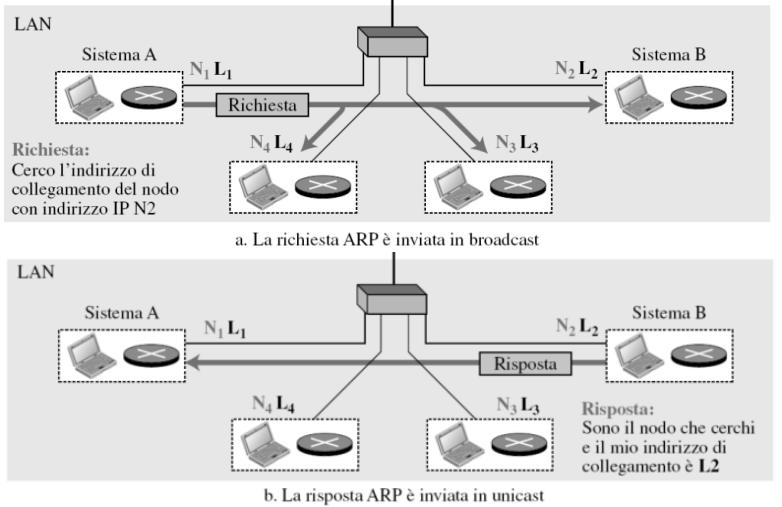
\includegraphics[width=0.6\textwidth]{images/funzionamento-arp.png}
        %\captionof{figure}{Percorso a costo minimo e tabella di inoltro per il nodo $u$}
    \end{minipage}
    
    Il sistema A deve passare il pacchetto al suo livello di collegamento per la consegna vera e propria, ma non conosce l'indirizzo fisico (indirizzo di collegamento) del ricevente. Esso quindi utilizza i servizi di ARP, chiedendo al protocollo di inviare in broadcast un pacchetto di richiesta, per scoprire l'indirizzo fisico del un sistema che ha N2 come indirizzo IP.

    Il pacchetto di richiesta ARP viene ricevuto da ogni sistema sulla rete fisica, ma solo il sistema B risponde, come mostrato nella figura, inviando un pacchetto di risposta ARP che contiene il suo indirizzo fisico. Ora il sistema A può inviare tutti i pacchetti che ha per tale destinazione, usando l'indirizzo fisico ottenuto per mezzo di ARP.
\end{Example}

\subsubsection{Formato del pacchetto ARP}
Viene mostrato il formato di un pacchetto ARP. I nomi dei campi spiegano da soli il loro significato. Il campo hardware type definisce il tipo del protocollo di livello collegamento che viene usato. Il campo protocol type definisce il protocollo del livello di rete.

\begin{figure}[ht]
    \centering
    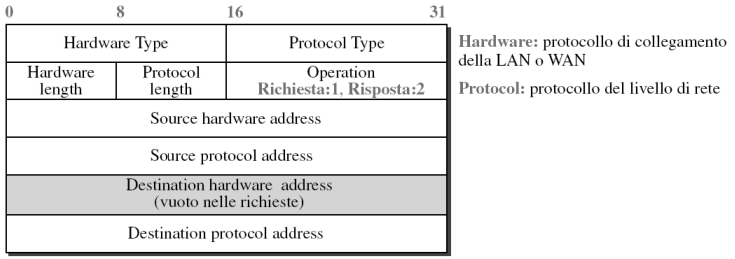
\includegraphics[width=11cm]{images/pacchetto-arp.PNG}
    \caption{Formato del pacchetto ARP}
    \label{fig:pacchetto-ARP}
\end{figure}

I campi source hardware address e source protocol address definiscono, per il mittente, il suo indirizzo fisico e quello del protocollo di livello superiore (IP nel nostro esempio). Entrambi i campi, per i motivi discussi in precedenza, sono di lunghezza variabile (lunghezze definite per mezzo di hardware length e protocol length). I campi destination hardware address e destination protocol address definiscono l'indirizzo fisico e quello del protocollo di livello superiore, ma in questo caso per il ricevente. I pacchetti ARP vengono incapsulati direttamente all'interno dei frame di livello collegamento. Per questo motivo il frame dovrà indicare all'interno della sua intestazione che trasporta un pacchetto ARP invece di un datagramma del livello di rete.



\begin{Example}{Pacchetto ARP}{}
    \textit{Un host con indirizzo IP N1 e indirizzo MAC (indirizzo fisico) L1 ha un pacchetto da inviare a un altro host con indirizzo IP N2 e indirizzo fisico L2 (indirizzo fisico che al momento è sconosciuto al primo host). I due host si trovano all'interno della stessa rete. Mostrare il pacchetto di richiesta ARP e quello di risposta, racchiusi all'interno dei frame Ethernet.}

    \begin{minipage}{\textwidth}
        \centering
        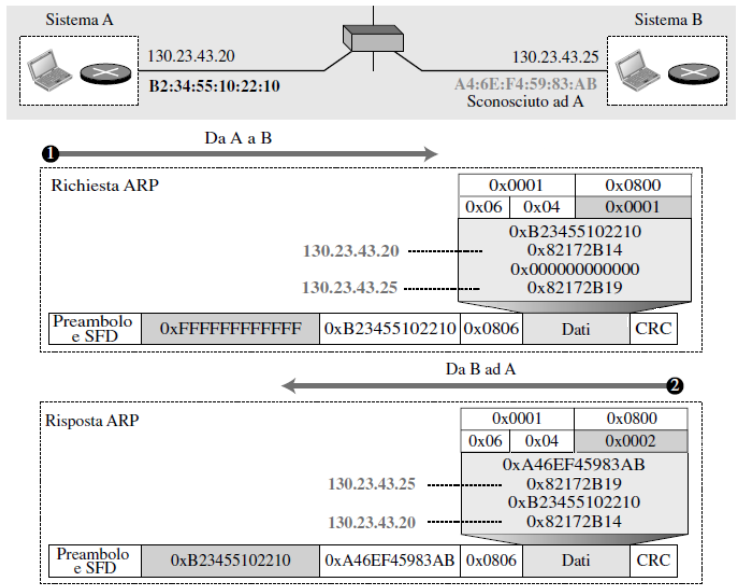
\includegraphics[width=0.6\textwidth]{images/es-pacchetto-arp.PNG}
        %\captionof{figure}{Percorso a costo minimo e tabella di inoltro per il nodo $u$}
    \end{minipage}

    La figura mostra la richiesta ARP e il pacchetto di risposta. Da notare che il campo dati ARP è in questo caso di 28 byte e che i vari indirizzi contenuti al suo interno hanno lunghezze differenti: 32 bit per IPv4 e 48 bit per Ethernet. Inoltre, in questo caso anche gli indirizzi IP sono rappresentati in esadecimale.
\end{Example}

Si è parlato di indirizzamento nei quattro livelli superiori della pila TCP/IP. A livello fisico invece non c'è alcun indirizzamento visto che questo livello si occupa di trasferire i singoli bit, che vengono spediti in broadcast nel mezzo trasmissivo e ricevuti da tutti i nodi che sono collegati a tale mezzo. Vediamo ora gli indirizzi dei vari livelli nell'ambito di un'unica transazione, così da poter fare attenzione alle varie interrelazioni che ci sono tra di loro. Vediamo anche come tutti questi indirizzi possono essere ricavati automaticamente dal sistema, purché sia noto il nome del sito che l'utente intende contattare. 

\begin{Example}{Indirizzamento}{}
    \textit{La figura mostra una internet semplificata dove ci sono Gaia e Gabriele. Gaia è un'utente che vuole accedere alla lista dei prodotti offerti da Gabriele. Gabriele ha una piccola attività chiamata \texttt{dagabriele.biz}, la lista dei prodotti e le relative specifiche sono memorizzate in un documento chiamato prodotti. }

    \begin{minipage}{\textwidth}
        \centering
        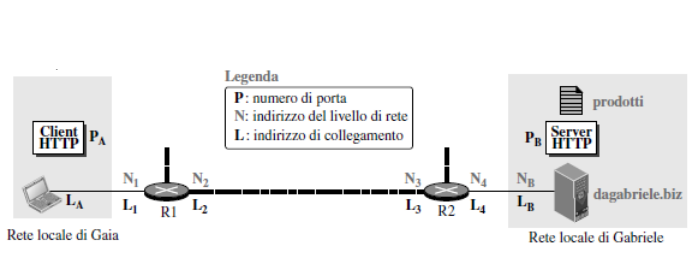
\includegraphics[width=0.7\textwidth]{images/es-arp1.PNG}
        %\captionof{figure}{Percorso a costo minimo e tabella di inoltro per il nodo $u$}
    \end{minipage}
    
    L'unico identificatore che Gaia deve conoscere è l'URL del sito che vuole visitare: \texttt{http://dagabriele.biz/prodotti}. Il resto degli indirizzi, sorgente e destinazione, vengono ricavati dal sistema, come mostriamo in questo esempio.

    Supponiamo che Gaia sia collegata ad una LAN e che il suo computer conosca sia il suo indirizzo IP che quello di collegamento. Anche il server di Gabriele è collegato ad una LAN (una diversa rispetto a quella di Gaia) ed anche il suo computer conosce entrambi i suoi indirizzi. La stessa cosa vale per i router all'interno della internet semplificata ciascun router conosce i propri indirizzi di rete e di collegamento. Nell'esempio verranno utilizzati degli indirizzi simbolici per rendere più leggibili le figure. Come spiegato in precedenza, Gaia non ha alcuna necessità di conoscere questi indirizzi: essi vengono ottenuti automaticamente nel corso della transazione.

    \begin{minipage}{\textwidth}
        \centering
        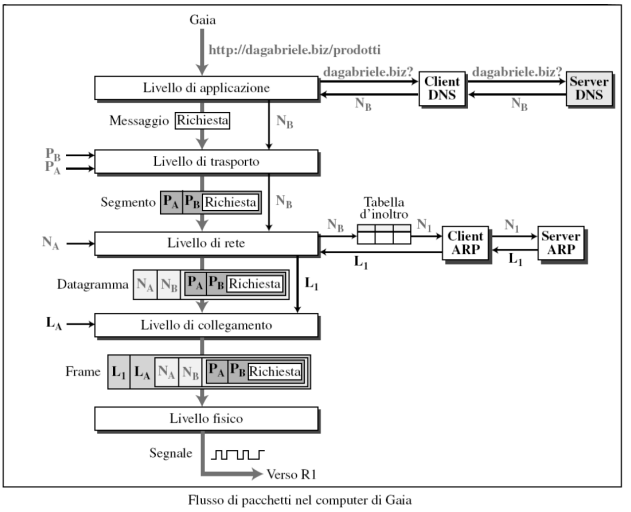
\includegraphics[width=0.6\textwidth]{images/es-arp2.PNG}
        %\captionof{figure}{Percorso a costo minimo e tabella di inoltro per il nodo $u$}
    \end{minipage}

    La figura mostra il flusso di pacchetti generati dal computer di Gaia. Gaia, usando un browser, digita l'URL del sito di Gabriele (\texttt{http://dagabriele.biz/prodotti}). Il computer di Gaia usa il client HTTP per soddisfare la sua richiesta. Il client HTTP, tuttavia, non conosce l'indirizzo IP di Gabriele, quindi chiama il client DNS per ottenere aiuto. Il client DNS invia una richiesta ad un server DNS e trova l'indirizzo IP del computer di Gabriele ($N_{B}$) che viene passato al livello trasporto.

    A questo punto il livello trasporto crea un segmento utilizzando il numero di porta noto del server HTTP ($P_B=80$) e un numero di porta temporaneo ottenuto dal sistema operativo ($P_A$) per il client HTTP. Ora il livello trasporto può predisporre un segmento e passarlo al livello di rete assieme all'indirizzo IP del computer di Gabriele ($N_{B}$), che è stato ottenuto nel passaggio precedente.

    Il livello di rete riceve il segmento e l'indirizzo di rete $N_{B}$. Il livello di rete consulta la sua tabella d'instradamento e cerca il router successivo a cui instradare il datagramma che è destinato all'indirizzo $N_{B}$. La risposta in questo caso è il router di default della rete in cui si trova Gaia e quindi la tabella di routing fornisce l'indirizzo $N_{1}$. Ma questo non è sufficiente, il livello di collegamento di Gaia ha la necessità di trovare l'indirizzo di collegamento del router R1. Utilizza quindi il suo client ARP per trovare l'indirizzo di collegamento $L_{1}$. Il livello di rete può ora passare il datagramma con l'indirizzo di collegamento giusto al livello di collegamento.

    Come detto in precedenza, il livello di collegamento di Gaia conosce il suo indirizzo di collegamento, $L_A$. Crea quindi il frame e lo passa al livello fisico dove viene convertito in segnali e spedito attraverso il mezzo trasmissivo.

    Ora vediamo cosa succede nel router R1. Come sappiamo, i router normalmente lavorano solamente ai tre livelli inferiori della pila TCP/IP. Il pacchetto ricevuto da una delle interfacce deve quindi salire tutti e tre questi livelli, ridiscenderli e poi essere spedito da un'altra interfaccia. 

    \begin{minipage}{\textwidth}
        \centering
        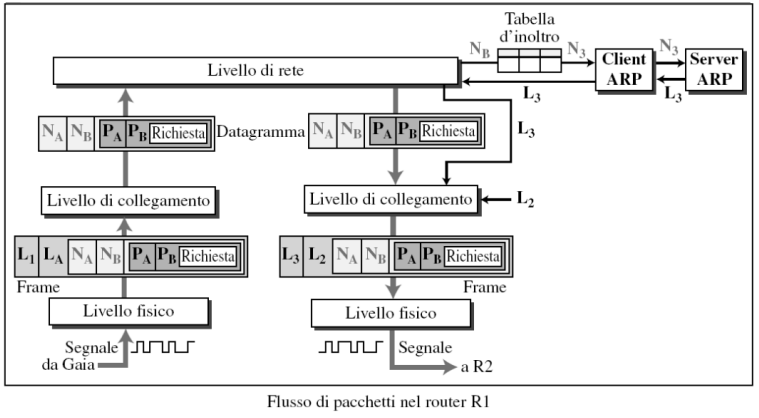
\includegraphics[width=0.6\textwidth]{images/es-arp3.PNG}
        %\captionof{figure}{Percorso a costo minimo e tabella di inoltro per il nodo $u$}
    \end{minipage}
    
    La figura mostra quanto avviene nel router. All'arrivo, il livello fisico del collegamento di sinistra (la rete a cui è collegata Gaia) riceve il frame e lo passa al livello di collegamento, che estrae il datagramma e lo passa al livello di rete. Esso esamina l'indirizzo del livello di rete del datagramma e scopre che deve essere consegnato al dispositivo con indirizzo IP $N_{B}$ Il livello di rete consulta la sua tabella d'inoltro per scoprire qual'è il nodo successivo (router) nel percorso verso $N_{B}$. La tabella d'inoltro restituisce $N_{3}$. L'indirizzo IP del router R2 indica che R2 si trova sullo stesso collegamento con R1. Il livello di rete di R1 ora usa ARP per trovare l'indirizzo di collegamento di R2, che risulta essere $L_{3}$ quindi passa il datagramma e l'indirizzo $L_{3}$ al livello di collegamento (lato destro del router R1). Il livello di collegamento incapsula il datagramma in un frame, aggiunge L3 e L2 (il suo indirizzo di collegamento sul lato destro) e passa il frame al livello fisico, che codifica i bit in segnali e li invia attraverso il mezzo trasmissivo a R2.

    Le attività nel router R2 sono le stesse del router R1, ad eccezione del fatto che alcuni indirizzi sono diversi.

    Ora vediamo cosa succede nella rete di Gabriele. 

    \begin{wrapfigure}{r}{0.32\textwidth}
        \vspace{-1cm}
        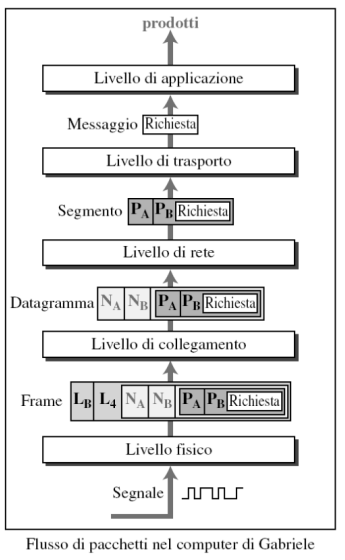
\includegraphics[width=0.30\textwidth]{images/es-arp4.PNG}
        \vspace{-1cm}
    \end{wrapfigure}
    
    La figura mostra come i segnali del livello fisico nell'host di Gabriele vengono tradotti in un messaggio destinato al programma server HTTP. Nella rete locale di Gabriele non servono più indirizzi o risoluzioni di indirizzi. Il segnale ricevuto dal collegamento viene tradotto in un frame, che viene passato al livello di collegamento, il quale estrae il datagramma e lo passa al livello di rete. Quest'ultimo estrae il segmento e lo passa al livello trasporto, che apre il segmento e passa il messaggio contenuto alla socket in ascolto sulla porta $P_B$(80). Il server HTTP riceve il messaggio, prepara una copia del file con i prodotti, lo trasforma in un documento HTML e lo restituisce a Gaia usando lo stesso flusso, ma in ordine inverso. Non è certo, ma il messaggio di ritorno probabilmente passerà attraverso i medesimi router, R2 e R1, per raggiungere Gaia.
\end{Example}

\section{LAN cablate: Ethernet}
Nel 1985, la IEEE Computer Society (Institute of Electrical and Electronics Engineers) iniziò un progetto, chiamato Progetto 802, con l'obiettivo di definire uno standard per l'interconnessione tra dispositivi di produttori differenti. Il Progetto 802 non aveva lo scopo di sostituire una qualsiasi parte del modello OSI o la pila TCP/IP, ma piuttosto intendeva definire chiaramente le funzioni specifiche del livello fisico e di collegamento dei protocolli LAN. Questo lavoro ha portato alla definizione dell'IEEE Standard 802.

L'IEEE ha suddiviso il livello di collegamento in due sotto-livelli: Logical Link Control (LLC) e Media Access Control (MAC). Inoltre, l'IEEE ha creato anche vari standard relativi ai livelli fisici delle tecnologie LAN.

\begin{figure}[ht]
    \centering
    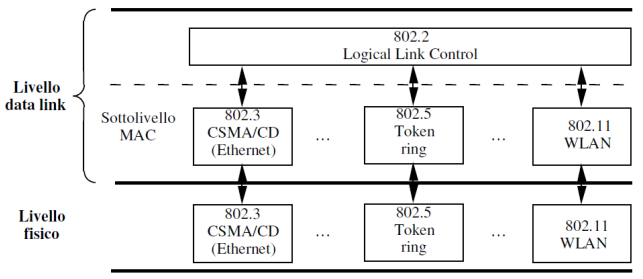
\includegraphics[width=11cm]{images/ieee-802.PNG}
    \caption{Gli standard IEEE per le LAN}
    \label{fig:ieee-802}
\end{figure}

In precedenza si è parlato del Data Link Control e in particolare si è detto che questo sotto-livello fornisce i servizi di framing, controllo di flusso e controllo degli errori. Nel caso di IEEE 802, il controllo di flusso, il controllo errori e parte delle funzioni di framing sono raccolte in un unico sotto-livello, chiamato Logical Link Control (LLC). Più in dettaglio il framing viene gestito sia nel sotto-livello LLC che all'interno del sotto-livello MAC.

Uno dei vantaggi di LLC è il fatto che fornisce un singolo protocollo di controllo del livello di collegamento comune per tutte le LAN definite dall'IEEE. In altri termini, questo significa che grazie al protocollo LLC è possibile avere interoperabilità tra diverse tecnologie LAN. Questo è possibile dal momento che LLC rende il sotto-livello MAC trasparente (cioè invisibile) al livello superiore.

Si è visto in precedenza che esistono diversi approcci per l'accesso multiplo al canale condiviso: accesso casuale, accesso controllato e suddivisione in canali. L'IEEE 802 ha definito un sotto-livello chiamato Media Access Control (MAC, controllo dell'accesso al mezzo trasmissivo) che definisce il metodo d'accesso specifico per ciascuna tipologia di LAN. Ad esempio, il MAC per le LAN Ethernet è il CSMA/CD. Infine, come si è detto poco sopra, parte del framing è compito del livello MAC.

Ethernet detiene una posizione dominante nel mercato delle LAN cablate. E' stata la prima LAN ad alta velocità con vasta diffusione. Sempre al passo dei tempi con il tasso trasmissivo: 10 Mbps (Ethernet standard) - 10 Gbps (10 Gigabit Ethernet).

\subsection{Ethernet standard}
Il frame Ethernet contiene sette campi:
\begin{figure}[ht]
    \centering
    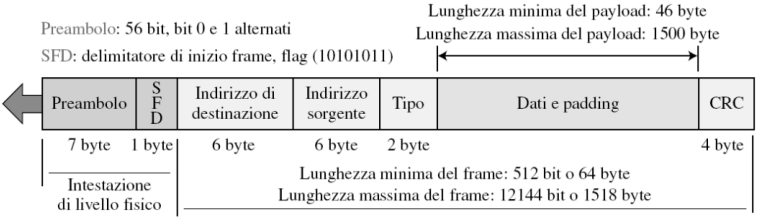
\includegraphics[width=11cm]{images/struttura-ethernet.PNG}
    \caption{Struttura dei frame Ethernet}
    \label{fig:struttura-ethernet}
\end{figure}

\begin{itemize}
    \item \textit{Preamble (preambolo).} Questo campo (7 byte quindi 56 bit) è composto da una serie di bit con valori 0 e 1 alternati. Il suo compito è quello di allertare il sistema ricevente circa l'arrivo del frame e permettere di sincronizzare il suo orologio con la trasmissione, nel caso non lo sia già. Il preambolo viene aggiunto a livello fisico e quindi non è propriamente parte del frame
    \item \textit{Start Frame Delimiter (SFD, delimitatore di inizio frame).} Questo campo (1 byte 10101011) segnala l'inizio del frame. L'SFD avverte la stazione o le stazioni riceventi che questa è la loro ultima possibilità di sincronizzazione. Gli ultimi 2 bit sono (11), e avvisano il ricevente che il campo seguente è l'indirizzo di destinazione. Quindi, in pratica, si tratta di un flag che definisce l'inizio del frame. Occorre ricordare che un frame Ethernet ha lunghezza variabile, quindi è necessario un flag per indicare l'inizio dei frame. Anche il campo SFD viene aggiunto dal livello fisico.
    \item \textit{Destination Address (DA, Indirizzo di destinazione).} Il campo (6 byte quindi 48 bit) contiene l'indirizzo di collegamento della stazione o delle stazioni destinatarie del frame. Quando la stazione ricevente trova in questo campo il suo stesso indirizzo di livello collegamento (unicast), l'indirizzo multicast di un gruppo di cui fa parte, o l'indirizzo broadcast, estrae i dati dal frame e li passa al protocollo di livello superiore (definito dal valore del campo Type).
    \item \textit{Source Address (SA, indirizzo della sorgente).} Anche questo campo è di 6 byte e contiene l'indirizzo di collegamento del mittente del frame.
    \item \textit{Type (Tipo).} Questo campo definisce il protocollo di livello superiore del pacchetto incapsulato all'interno del frame. Il protocollo può essere IP, ARP, OSPF e così via. E' quindi necessario per il multiplexing e il de-multiplexing a livello di collegamento.
    \item \textit{Data and padding (Dati).} Questo campo trasporta i dati incapsulati nel frame dai protocolli di livello superiore. Ha un minimo di 46 byte e un massimo di 1500 byte. Se i dati che provengono dal livello superiore superano i 1500 byte, essi devono essere frammentati e quindi racchiusi in più frame. Se sono meno di 46 byte, è necessario aggiungere tanti 0 quanti sono necessari per arrivare alla dimensione minima (padding). Una volta decapsulati i dati contenuti nel frame vengono consegnati così come sono al protocollo di livello superiore, quindi senza rimuovere il padding (gli 0 aggiuntivi).
    \item \textit{CRC.} L'ultimo campo contiene informazioni per il rilevamento errori. Il codice di ridondanza contenuto in questo campo viene calcolato sui campi indirizzo, tipo e dati. Se il ricevente lo calcola e constata che non è 0, allora il frame è stato alterato durante la trasmissione, e quindi il ricevente si limita a scartarlo.
\end{itemize}

\subsubsection{Servizio senza connessione e inaffidabile}
Ethernet fornisce un servizio senza connessione, questo significa che ogni frame inviato è indipendente dal frame precedente e dal successivo. In Ethernet non c'è alcuna fase di apertura o chiusura della connessione, il mittente si limita ad inviare un frame ogni volta che ne ha uno pronto, indipendentemente dal fatto che il destinatario sia pronto o meno a riceverlo. Può accadere che il mittente sommerga il ricevente di frame, con il risultato che alcuni di questi vengano scartati. Nel caso in cui un frame venga scartato, il mittente non viene informato dell'accaduto.

L'inaffidabilità di Ethernet è pari a quella di IP e UDP. Se un frame viene danneggiato durante la trasmissione e il ricevente riscontra il danneggiamento (grazie al codice di ridondanza contenuto nell'intestazione del frame), il ricevente si limiterà a scartare il frame, senza alcun'altra azione. E' dovere dei protocolli di livello superiore riscontrare la perdita dei dati e porvi rimedio.

\subsubsection{Lunghezza del frame}
Ethernet impone delle restrizioni sulla lunghezza minima dei frame e su quella massima. La restrizione sulla lunghezza minima è necessaria per il corretto funzionamento del meccanismo CSMA/CD. Un frame Ethernet deve avere una lunghezza minima di 512 bit (64 byte). Parte di questa lunghezza è relativa all'intestazione (header) e al trailer (la parte di frame che segue il campo dati). Se contiamo 18 byte di intestazione e trailer (6 byte di indirizzo della sorgente, 6 byte di indirizzo di destinazione, 2 byte per il Tipo e 4 byte di CRC), la lunghezza minima dei dati che il livello superiore deve fornire è 64-18 = 46 byte. Se il pacchetto di livello superiore ha dimensione inferiore ai 46 byte, vengono aggiunti dei bit di riempimento per compensare la differenza (padding).

Lo standard Ethernet definisce la lunghezza massima del frame (senza contare il preambolo e il campo SFD) a 1518 byte. Se vengono sottratti i 18 byte dell'intestazione e del trailer, la lunghezza massima dei dati è 1500 byte. Questa restrizione deriva da due ragioni storiche: in primo luogo, la memoria, quando è stato inventata Ethernet, era molto costosa. Quindi questa restrizione permetteva di ridurre la dimensione dei buffer nei dispositivi. In secondo luogo essa evita che una stazione possa monopolizzare il mezzo trasmissivo condiviso, impedendo alle altre stazioni di inviare i loro frame.

\subsubsection{Indirizzi}
Tutte le stazioni che fanno parte di una rete Ethernet (ad esempio un computer, una postazione di lavoro o una stampante) sono dotate di una Network Interface Card (NIC), comunemente detta scheda di rete. La NIC viene installata nella stazione e fornisce un suo indirizzo di livello collegamento. Gli indirizzi Ethernet sono composti da 6 byte (48 bit) e vengono normalmente scritti in notazione esadecimale, con i due punti a dividere i vari byte.

Quando gli indirizzi Ethernet vengono trasmessi, la loro codifica è diversa rispetto a come vengono rappresentati quando vengono scritti. Infatti, gli indirizzi vengono trasmessi da sinistra a destra, byte per byte, ma per ciascun byte il bit meno significativo viene inviato per primo e quello più significativo per ultimo. Grazie a questo semplice meccanismo il ricevente è in grado di capire già dal primo bit se il frame che sta ricevendo è unicast o multicast.

\subsubsection{Metodo di accesso}
Dato che il protocollo Ethernet Standard utilizza un approccio broadcast, era necessario implementare un metodo di accesso al mezzo trasmissivo condiviso. La modalità usata dall'Ethernet Standard era quella del CSMA/CD con il metodo dell'1 persistente. Per mezzo di un semplice esempio vediamo questi meccanismi applicati ad Ethernet.

\begin{Example}{Fasi operative del protocollo CSMA/CD}{}
    \textit{Supponiamo che la stazione A nella figura abbia un frame da inviare alla stazione D.}
    
    \begin{minipage}{\textwidth}
        \centering
        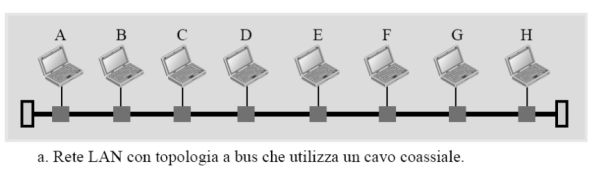
\includegraphics[width=0.6\textwidth]{images/ethernet-standard.PNG}
        %\captionof{figure}{Percorso a costo minimo e tabella di inoltro per il nodo $u$}
    \end{minipage}
    
    Per prima cosa la stazione A dovrebbe verificare se c'è un'altra stazione che sta già tra smettendo (carrier sense). Per far questo misura il livello di energia sul mezzo trasmissivo per un breve periodo di tempo (normalmente meno di $100\mu s$). L'assenza di segnale significa che nessuna stazione sta inviando (o il segnale non ha ancora raggiunto la stazione A). La stazione interpreta questa situazione come "mezzo inattivo" ed inizia a inviare il suo frame. Se invece rileva la presenza di segnale, questo significa che il mezzo trasmissivo è attualmente utilizzato da un'altra stazione. La stazione A controlla continuamente il mezzo finché non rimane inattivo per $100 \mu s$, quindi inizia a inviare il suo frame. La stazione non può immediatamente gettare il frame, deve tenerne una copia nel buffer fino a quando non è sicura che non vi sia stata una collisione.

    Il rilevamento del mezzo trasmissivo non può fermarsi dopo che la stazione A ha iniziato a inviare il frame, è necessario che continui a rimanere in ascolto anche mentre invia il frame. Possono verificarsi due casi:
    \begin{enumerate}
    \item La stazione A ha inviato 512 bit e non ha rilevato alcuna collisione; la stazione è quindi certa che il frame sia stato inviato senza collisioni ed interrompe la rilevazione sul mezzo trasmissivo. Da dove proviene la dimensione 512 bit? Considerando la velocità di trasmissione di Ethemet pari a 10 Mbps, questo significa che alla stazione occorrono 512/(10 Mbps) = 51,2 µs per inviare 512 bit. Con la velocità di propagazione in un cavo pari a 2 x 10 metri, il primo bit può aver percorso 10240 metri (solo andata) o 5120 metri (nel caso di andata e ritorno), aver avuto una collisione con un bit della stazione più lontana sul cavo ed essere tornato indietro. In altre parole, se si verifica una collisione, questa deve avvenire entro il momento in cui il mittente ha inviato 512 bit (caso peggiore) e il primo bit ha effettuato un'andata e ritorno di 5120 metri. Nel caso la collisione avvenga a metà del cavo, e non alla fine, la stazione rileverà la collisione ed interromperà la trasmissione.
    \item La stazione A ha rilevato una collisione prima di inviare 512 bit. Ciò significa che uno dei precedenti bit è andato in collisione con un bit inviato da un'altra stazione. In questo caso entrambe dovrebbero astenersi dal trasmettere e mantenere il frame nei loro buffer per reinviarlo quando il mezzo trasmissivo sarà disponibile. Tuttavia, per informare le altre stazioni nella rete che vi è una collisione, la stazione invia un segnale di disturbo formato da 48 bit, che serve a creare sufficiente segnale (anche se la collisione avviene dopo pochi bit) per allertare le altre stazioni della collisione. Dopo l'invio del segnale di disturbo, la stazione deve incrementare il valore di $K$ (numero di tentativi). Se, dopo l'incremento, $K$ ha raggiunto il valore 15, allora si può assumere che la rete al momento sia troppo congestionata. La stazione quindi dovrebbe abbandonari suoi sforzi e riprovare solamente più tardi. Se $K < 15$ la stazione può aspettare un tempo di back-off e riavviare il procedimento. La stazione genera un numero casuale compreso tra 0 e $2 ^K - 1$ che significa che ogni volta che avviene una collisione l'intervallo dei numeri casuali cresce in modo esponenziale. Dopo la prima collisione ($K = 1$) il numero casuale viene scelto nell'intervallo (0, 1). Dopo la seconda ($K = 2$) tra (0, 1, 2, 3), dopo la terza ($K = 3$) tra (0, 1, 2, 3, 4, 5, 6, 7). Quindi dopo ciascuna collisione, aumenta la probabilità che il tempo di back-off diventi maggiore. Ciò è dovuto al fatto che se la collisione avviene anche dopo il terzo o il quarto tentativo, significa che la rete è molto occupata, occorre quindi attendere per un tempo di back-off più lungo.
    \end{enumerate}
\end{Example}

\subsection{Fast Ethernet (100 Mbps}
Negli anni novanta sul mercato apparvero alcune tecnologie LAN con velocità di trasmissione superiore a 10 Mbps (come ad esempio FDDI e Fiber Channel). Ethernet quindi doveva competere con queste nuove tecnologie e la sua sopravvivenza era legata alla sua capacità di aumentare la velocità di trasferimento. L'evoluzione di Ethernet Standard, chiamata Fast Ethernet, ha fatto un notevole salto giungendo a ben 100 Mbps. Uno dei requisiti fondamentali in questa evoluzione era la necessità di mantenere Fast Ethernet compatibile con la versione precedente. Per questo motivo il sotto-livello MAC rimase del tutto immutato, questo significa che anche il formato del frame e le sue dimensioni (massima e minima) rimasero invariati. Con l'aumento della velocità di trasmissione, fu necessario riconsiderare alcune caratteristiche dell'Ethernet Standard che dipendono dalla velocità di trasmissione, ad esempio il metodo d'accesso.

\subsubsection{Metodo di accesso}
E' bene ricordare che il funzionamento corretto del CSMA/CD dipende dalla velocità di trasmissione, dalla dimensione minima del frame e dalla lunghezza massima della rete. Se si vuole mantenere inalterata la dimensione minima del frame è quindi necessario modificare la lunghezza massima della rete. In altre parole, se la dimensione minima del frame è ancora 512 bit e la trasmissione è 10 volte più veloce, allora le collisioni devono essere rilevate 10 volte più velocemente. Tutto questo porta al fatto che la rete dovrebbe essere 10 volte più corta (la velocità di propagazione ovviamente non cambia). Per questo motivo sono state previste due diverse soluzioni per il funzionamento di Fast Ethernet.
\begin{enumerate}
    \item La prima soluzione è quella di abbandonare la topologia a bus, utilizzare un hub passivo con una topologia stella, ma fissare la dimensione massima della rete a 250 metri invece dei 2500 della versione Standard.
    \item La seconda soluzione prevede l'uso di un commutatore di livello collegamento, detto anche switch dotato di buffer per memorizzare i frame e una connessione full-duplex (bi-direzionale) per ciascun host. In questo modo, in pratica, il mezzo trasmissivo è privato per ciascun host e non c'è alcuna ragione per usare il CSMA/CD, dal momento che gli host non sono più in competizione tra loro per accedere al mezzo trasmissivo. Lo switch riceve un frame da un host sorgente e lo memorizza nel buffer (coda) in attesa di elaborazione. Successivamente verifica l'indirizzo di destinazione e invia il frame attraverso l'interfaccia corrispondente. Dal momento che il collegamento al commutatore è full-duplex, il commutatore può persino inviare un frame a una destinazione mentre riceve un altro frame da un'altra stazione. In altre parole, il singolo mezzo trasmissivo condiviso è stato modificato in molti mezzi trasmissivi punto-punto e senza necessità di contesa.
\end{enumerate}

\subsection{Gigabit Ethernet}
Il bisogno di velocità di trasferimento ancora maggiori ha portato alla progettazione di Gigabit Ethernet (1000 Mbps). Come è evidente anche dal nome, lo scopo di Gigabit Ethernet era quello di aggiornare la velocità di trasferimento dati a 1 Gbps mantenendo invariata la lunghezza dell'indirizzo, il formato e la lunghezza massima e minima dei frame.

La topologia delle reti Gigabit Ethernet prevede la presenza di uno switch al centro della stella, e tutti i computer (o altri switch) collegati ai vari rami della stella. Lo switch, per ogni porta, prevede la presenza di buffer dove i frame vengono memorizzati prima di essere trasmessi. Anche in questo caso, il mezzo trasmissivo tra le stazioni e lo switch centrale è privato, non ci sono collisioni e quindi non c'è alcuna necessità di usare CSMA/CD. L'assenza di collisioni implica che la massima lunghezza del cavo non è più determinata dal meccanismo di rilevazione delle collisioni bensi solo dall'attenuazione del segnale.

\subsection{10-Gigabit Ethernet}
Negli ultimi anni è stata predisposta un'ulteriore revisione di Ethernet per l'uso nelle MAN (Metropolitan Area Network). L'idea alla base in questo caso è quella di estendere la tecnologia, la velocità di trasferimento dei dati e la distanza massima di copertura affinché Ethernet possa essere usata sia come LAN che come MAN, quindi su aree decisamente più vaste che in passato.

\subsection{LAN virtuali}
Una stazione è considerata parte di una LAN se ne fa fisicamente parte. Che cosa accade se occorre un "collegamento virtuale" tra due stazioni che appartengono a due LAN fisiche diverse? In maniera piuttosto generale possiamo definire una Virtual Local Area Network (VLAN) come una rete locale configurata per mezzo del software, anziché del cablaggio fisico.

\begin{Example}{Uno switch che supporta le VLAN}{}
    \textit{Nella figura viene mostrato un esempio di LAN commutata, ad esempio una piccola ditta, dove 10 stazioni sono raggruppate in 3 LAN e queste ultime sono interconnesse per mezzo di uno switch.}

    \begin{minipage}{\textwidth}
        \centering
        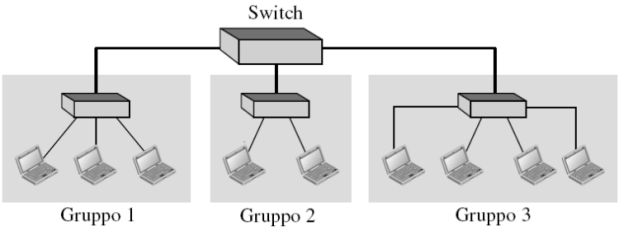
\includegraphics[width=0.6\textwidth]{images/lan-virtuali.PNG}
        %\captionof{figure}{Percorso a costo minimo e tabella di inoltro per il nodo $u$}
    \end{minipage}
    
    Il personale del primo gruppo lavora assieme, così come per il secondo ed il terzo gruppo. Ma cosa accade se c'è la necessità di spostare uno dei dipendenti del primo gruppo in un altro dei gruppi? E' necessario modificare la configurazione delle LAN, o più in dettaglio è necessario modificare i cavi di collegamento tra le varie stazioni, quindi sono necessari dei cambi fisici alla topologia di rete.

    \begin{minipage}{\textwidth}
        \centering
        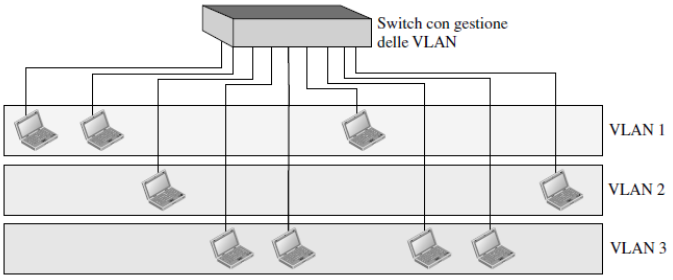
\includegraphics[width=0.6\textwidth]{images/vlan.PNG}
        %\captionof{figure}{Percorso a costo minimo e tabella di inoltro per il nodo $u$}
    \end{minipage}
    
    La figura mostra la stessa LAN suddivisa in VLAN. L'idea alla base della tecnologia VLAN è quella di dividere una LAN in segmenti logici, anziché fisici. Una LAN può essere quindi suddivisa in più LAN logiche chiamate VLAN. Nella pratica ciascuna di queste può rappresentare un gruppo di lavoro all'interno della ditta. Se un dipendente si sposta da un gruppo ad un altro, non c'è bisogno di cambiare la configurazione fisica. Nella VLAN il gruppo di appartenenza delle stazioni è definito dal software, non dall'hardware. Qualsiasi stazione può essere spostata facilmente da una VLAN ad un'altra. Tutti i membri appartenenti ad una VLAN possono ricevere i pacchetti broadcast inviati a questa particolare VLAN. Ciò significa che se una stazione si sposta dalla VLAN 1 alla VLAN 2, riceve i messaggi broadcast inviati alla VLAN 2, ma non riceve più quelli inviati alla VLAN 1.
\end{Example}

\section{Switch di livello collegamento}
Uno switch di livello collegamento (commutatore di livello collegamento) opera sia a livello fisico che a livello di collegamento. Come dispositivo di livello fisico rigenera il segnale che riceve. Inoltre, come dispositivo di livello collegamento, è in grado di verificare gli indirizzi MAC (sorgente e destinazione) contenuti nel frame.

E' normale chiedersi qual è la differenza di funzionalità tra uno switch e un hub. Il primo ha capacită di filtraggio (filtering), è in grado di verificare l'indirizzo di destinazione del frame e decidere da quale porta in uscita deve essere inviato il frame. Uno switch ha una tabella che viene utilizzata per il filtraggio.

Uno switch trasparente è un commutatore di cui le stazioni presenti nella rete sono completamente ignare dell'esistenza del dispositivo di rete. Se uno switch viene aggiunto o eliminato dalla rete, non è necessaria alcuna operazione di riconfigurazione delle stazioni.

\subsection{Apprendimento}
Inizialmente gli switch operavano usando della tabelle statiche di commutazione. Questo significa che l'amministratore di rete era costretto ad inserire manualmente ciascuna voce della tabella durante la configurazione dello switch. Nonostante il processo fosse abbastanza semplice, non era molto comodo. Infatti, se una stazione veniva aggiunta o cancellata, la tabella doveva essere modificata manualmente. La stessa cosa doveva essere fatta se l'indirizzo MAC di una stazione cambiava, un evento tutt'altro che raro (ad esempio per il cambio di una scheda di rete).

La soluzione, molto migliore della tabella statica, è una tabella dinamica che associa automaticamente gli indirizzi MAC alle porte (interfacce). Per creare una tabella dinamica, occorre uno switch che sia in grado di apprendere gradualmente dai frame che vengono inviati all'interno della rete. Per fare questo, lo switch analizza gli indirizzi sorgente e destinazione di ogni frame. L'indirizzo di destinazione viene utilizzato per decidere su quale interfaccia inoltrare il frame, quello sorgente invece serve per aggiungere nuove voci alla tabella e quindi, poco alla volta, configurarla automaticamente.

\begin{Example}{Switch con auto-apprendimento}{}
    \textit{Vediamo più in dettaglio questo procedimento utilizzando l'esempio della figura.}
    
    \begin{minipage}{\textwidth}
        \centering
        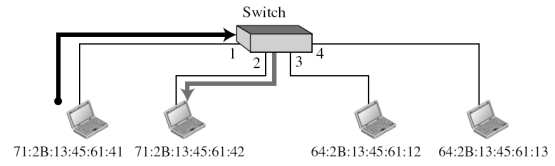
\includegraphics[width=0.6\textwidth]{images/es-switch.PNG}
        %\captionof{figure}{Percorso a costo minimo e tabella di inoltro per il nodo $u$}
    \end{minipage}
    \begin{enumerate}
    \item Quando la stazione A invia un frame alla stazione D, lo switch nella sua tabella non ha alcuna voce sia per D che per A. Il frame viene quindi inviato in broadcast su tutte le porte (ad esclusione di quella da cui è stato ricevuto). Analizzando l'indirizzo sorgente, lo switch apprende che la stazione A è collegata alla porta 1. Ciò indica che i frame destinati ad A, in futuro, dovranno essere inviati solo attraverso la porta 1. Lo switch aggiunge immediatamente questa informazione alla sua tabella, che ora contiene la sua prima voce.
    \item Quando la stazione D invia un frame alla stazione B, lo switch non ha una voce relativa a B, cosi invia nuovamente in broadcast il frame. Tuttavia, questo frame permette di aggiunge un'ulteriore voce alla tabella: la porta a cui è collegata la stazione D.
    \item Il processo di apprendimento continua fino a quando la tabella non contiene informazioni su tutte le stazioni e le relative porte. C'è da notare che il processo di apprendimento potrebbe richiedere molto tempo. Ad esempio, se una stazione non trasmette alcun frame essa non avrà mai una voce nella tabella, ma si tratta di una situazione estremamente improbabile.
    \end{enumerate}
\end{Example}

Gli switch sono dispositivi plug-and-play che non richiedono intervento dell’amministratore di rete o dell’utente. Eliminano le collisioni ovvero bufferizzano i frame e non trasmettono più di un frame alla volta su ogni segmento di rete, inoltre interconnettono link eterogenei cioè collegamenti che operano a diverse velocità possono essere collegati a uno switch. Aumentano la sicurezza della rete e migliorano il network management. Infine forniscono informazioni su uso di banda, collisioni, tipi di traffico...